% Copyright 2004 by Till Tantau <tantau@users.sourceforge.net>.
%
% In principle, this file can be redistributed and/or modified under
% the terms of the GNU Public License, version 2.
%
% However, this file is supposed to be a template to be modified
% for your own needs. For this reason, if you use this file as a
% template and not specifically distribute it as part of a another
% package/program, I grant the extra permission to freely copy and
% modify this file as you see fit and even to delete this copyright
% notice. 
\UseRawInputEncoding
\documentclass{beamer}

% There are many different themes available for Beamer. A comprehensive
% list with examples is given here:
% http://deic.uab.es/~iblanes/beamer_gallery/index_by_theme.html
% You can uncomment the themes below if you would like to use a different
% one:
%\usetheme{AnnArbor}
%\usetheme{Antibes}
%\usetheme{Bergen}
%\usetheme{Berkeley}
%\usetheme{Berlin}
%\usetheme{Boadilla}
%\usetheme{boxes}
%\usetheme{CambridgeUS}
%\usetheme{Copenhagen}
%\usetheme{Darmstadt}
%\usetheme{default}
%\usetheme{Frankfurt}
%\usetheme{Goettingen}
%\usetheme{Hannover}
%\usetheme{Ilmenau}
%\usetheme{JuanLesPins}
%\usetheme{Luebeck}
\usetheme{Madrid}
%\usetheme{Malmoe}
%\usetheme{Marburg}
%\usetheme{Montpellier}
%\usetheme{PaloAlto}
%\usetheme{Pittsburgh}
%\usetheme{Rochester}
%\usetheme{Singapore}
%\usetheme{Szeged}
%\usetheme{Warsaw}

\usepackage{ragged2e}
\usepackage{multicol}
\usepackage{pgfgantt}
%\usepackage{todonotes}
\usepackage{media9}
\usepackage{subfigure}
\usepackage{wrapfig}
% Customize Warsaw color 
\setbeamercolor*{palette primary}{use=structure,fg=white,bg=blue!50!black}
\setbeamercolor*{palette secondary}{use=structure,fg=white,bg=blue!60!black}
\setbeamercolor*{palette tertiary}{use=structure,fg=white,bg=blue!70!black}

% Customize Warsaw block title and background colors
\setbeamercolor{block title}{bg=red!50!black,fg=white}

\setbeamertemplate{bibliography item}{\insertbiblabel}  % insert bibliography numbers instead of symbol
\setbeamertemplate{caption}[numbered] % adds the figure or table number to the caption.

\usepackage{siunitx}
\sisetup{unitsep=\cdot}

\usepackage{tikz}
% load libraries
\usetikzlibrary{backgrounds,calc,patterns,decorations.pathmorphing,decorations.markings,shapes,arrows,snakes,tikzmark}
\usepackage[siunitx,smartlabels]{circuitikz}
\def\smgrid{0.5}
% For compact drawing of resistors and capacitors 1
\ctikzset{resistors/scale=0.5,
  capacitors/scale=0.6,
  sources/scale=0.9} 
\ctikzset{
  amplifiers/fill=cyan,
  sources/fill=green!50,
  diodes/fill=red,
  resistors/fill=violet,
}

\title[iBEMS]{Intelligent Building Energy Management System}

% % A subtitle is optional and this may be deleted
% \subtitle{Product Proposal}

\author[B.~Lauer, E.~Watkins]{Brian~Lauer \and Elliot~Watkins\\
Advisor: Dr. Suruz Miah}
% - Give the names in the same order as the appear in the paper.
% - Use the \inst{?} command only if the authors have different
%   affiliation.

\institute[Bradley University] % (optional, but mostly needed)
{
  Department of Electrical and Computer Engineering\\
  Bradley University\\
  1501 W. Bradley Avenue\\
  Peoria, IL, 61625, USA
}
% - Use the \inst command only if there are several affiliations.
% - Keep it simple, no one is interested in your street address.

%\date[November~27,~2018]{Tuesday, November~27,~2018}
\date[April~27,~2021]{Tuesday, April~27,~2021}
%\date[December~4,~2018]{Tuesday, December~4,~2016}

% - Either use conference name or its abbreviation.
% - Not really informative to the audience, more for people (including
%   yourself) who are reading the slides online

\logo{\hfill\href{http://www.bradley.edu}{
\includegraphics[width=0.75cm]{figs/logoBU1-Print}}}  % place logo in every page 

\subject{Building Energy Management}
% This is only inserted into the PDF information catalog. Can be left
% out. 

% If you have a file called "university-logo-filename.xxx", where xxx
% is a graphic format that can be processed by latex or pdflatex,
% resp., then you can add a logo as follows:

% \pgfdeclareimage[height=0.5cm]{university-logo}{university-logo-filename}
% \logo{\pgfuseimage{university-logo}}

% Delete this, if you do not want the table of contents to pop up at
% the beginning of each subsection:
\AtBeginSection[]
{
  \begin{frame}<beamer>{Outline}
    \tableofcontents[currentsection,currentsubsection]
  \end{frame}
}

% Let's get started
\begin{document}

\begin{frame}
  \titlepage
\end{frame}

\begin{frame}{Outline} %
  \tableofcontents%[pausesections]
  % You might wish to add the option [pausesections]
\end{frame}

% Section and subsections will appear in the presentation overview
% and table of contents.
\section{Introduction}

\begin{frame}{Introduction}{} % Elliot
    % Applications of Building Energy Management
    % \begin{multicols}{2}
      % \begin{block}{}
  \begin{columns}
    \column{0.45\textwidth}
    \begin{block}{}
      \begin{small}
        \begin{itemize}
        \item Problems that iBEMS will address
          \begin{itemize}
          \item Can help save on energy costs
          \item Less impact on environment
          \end{itemize}
        \item How can the IoT help?
          \begin{itemize}
          \item WiFi integrated into most buildings
          \item Our Web-based approach simplifies development and end-user experience
          \end{itemize}
        \end{itemize}
      \end{small}
    \end{block}
    \column{0.5\textwidth}
    {\small
      \begin{block}{Overall Goal}
        \begin{itemize}
        \item Create a platform in which users can login and access $2$ or $3$ IoT devices connected to a building's energy supply
        \item Allow user to closely monitor energy usage for residential building
        \end{itemize}
      \end{block}
      }
    \begin{figure}
      \centering
      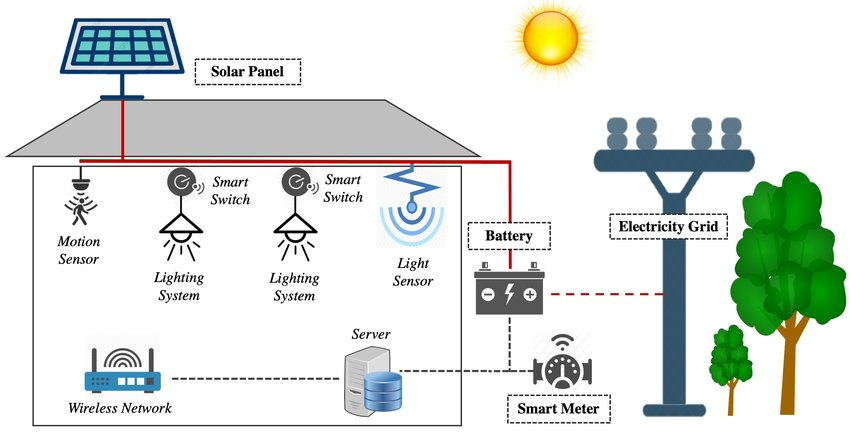
\includegraphics[scale=0.25]{figs/BEMS_Image.jpg}
      \caption{General BEMS}
      \label{fig:high_level_arch}
    \end{figure}
  \end{columns}
\end{frame}

\section{Architecture}
\begin{frame}{Architecture}{} % Brian
    \begin{columns}
        \column{0.5\textwidth}
        {\small
        \begin{figure}
            \centering
            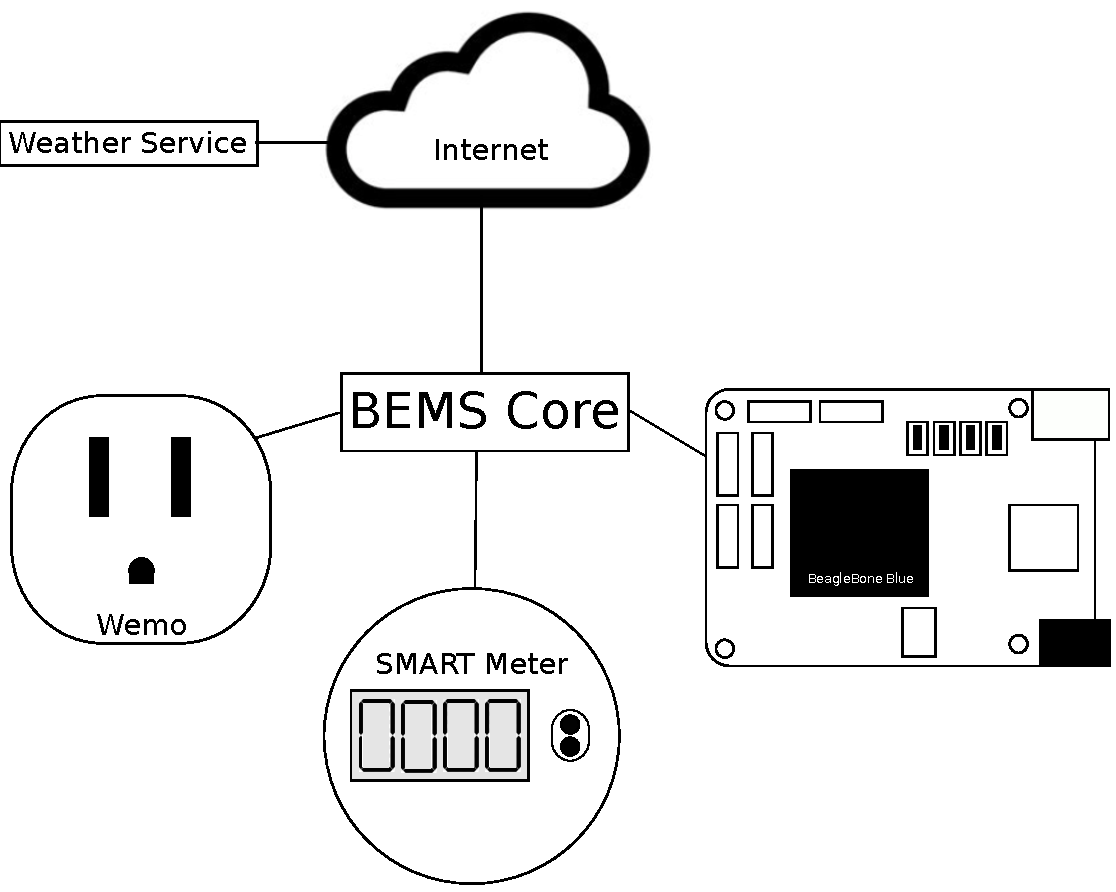
\includegraphics[scale=0.3]{figs/highLevelArchitecture.pdf}
            \caption{High Level Architecture}
            \label{fig:high_level_arch}
        \end{figure}
        }
        \column{0.45\textwidth}
        {\small
            \begin{block}{}
                \begin{itemize}
                    \item iBEMS currently has support for 2 IoT devices (WeMo Insight Switch and embedded computer) and can download weather data for the user
                    \item A microgrid with a smart meter could theoretically simulated and connected to by the BEMS core
                \end{itemize}
            \end{block}
        }
    \end{columns}
\end{frame}

\begin{frame}{Architecture}{} % Brian
    \begin{columns}
    \column{0.5\textwidth}
        \begin{figure}
            \centering
            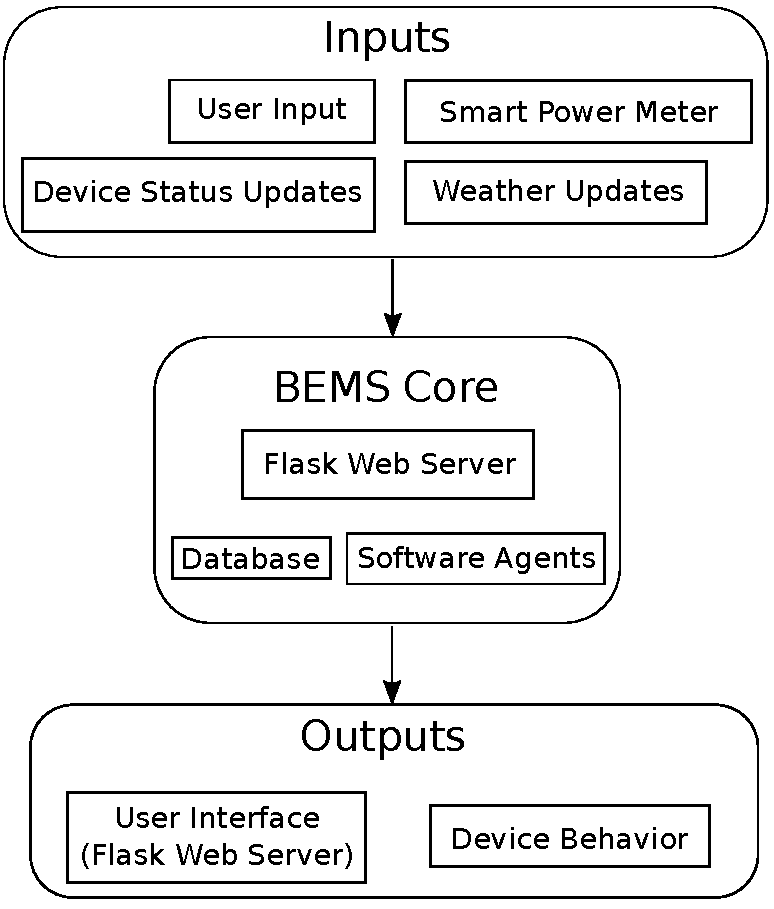
\includegraphics[scale=0.4]{figs/functionalBlockDiagram.pdf}
            \caption{Functional Block Diagram}
            \label{fig:functional_bd}
        \end{figure}
    \column{0.45\textwidth}
        \begin{block}{}
            \begin{small}
                \begin{itemize}
                    \item iBEMS receives input from users, connected devices, and will automatically download weather data
                    \item The core of iBEMS consists of a web server, a database and software agents which handle interactions with connected devices
                    \item Power data, device status, and schedules for each device will be output to the web server. Additionally, connected devices respond to commands from the iBEMS
                \end{itemize}
            \end{small}
        \end{block}
    \end{columns}
\end{frame}

\begin{frame}{Operational Modes}{}
    \begin{columns}
    \column{0.5\textwidth}
      \begin{figure}
        \centering
        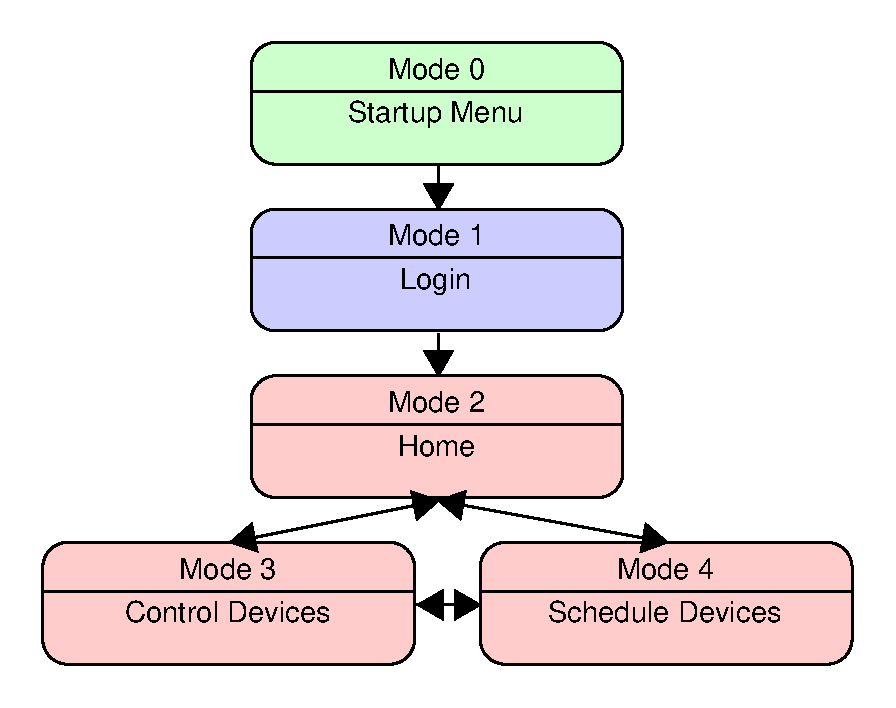
\includegraphics[scale=0.4]{figs/operationalModes.pdf}
        \caption{Operation Modes Interaction}
        \label{fig:functional_bd}
      \end{figure}
    \column{0.45\textwidth}
      \begin{block}{}
        \begin{enumerate}
            \setcounter{enumi}{-1}
            \item Startup menu
            \item Login - system administrators can add and configure users
            \item Home - view weather data
            \item Controlling devices
            \item Scheduling devices
        \end{enumerate}
    \end{block}
    \end{columns}
    
\end{frame}

\begin{frame}{Agent Communication Architecture}{}
    \begin{figure}
        \centering
        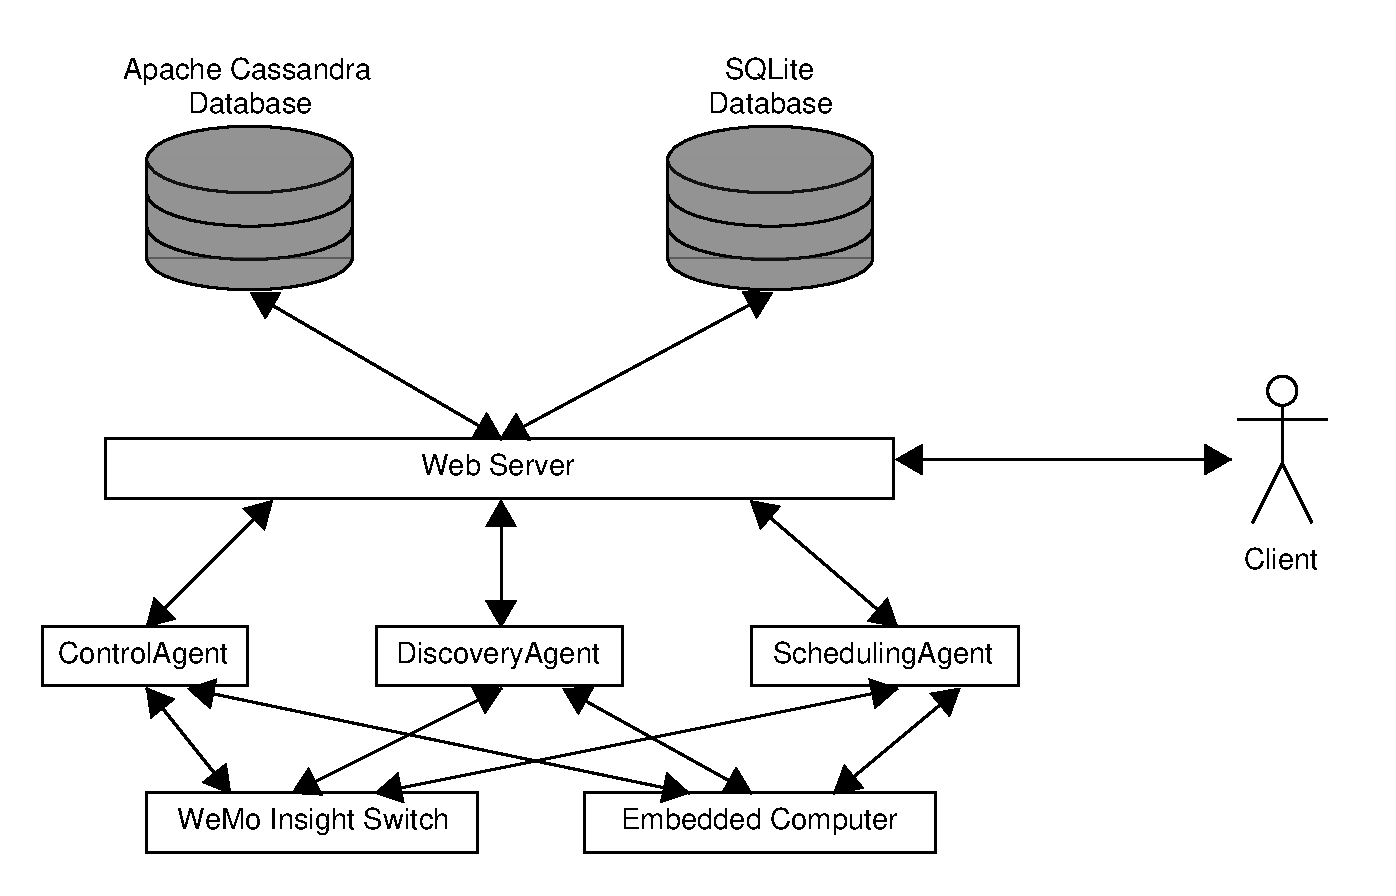
\includegraphics[scale=0.4]{figs/overallDiagram.pdf}
        \caption{Interconnection between system components}
        \label{fig:systemComponentInterconnection}
    \end{figure}
\end{frame}

\begin{frame}{Agent and Web Server Communication}{}
    \begin{figure}
        \centering
        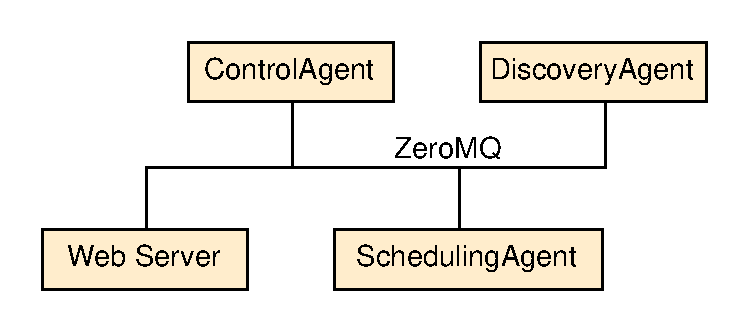
\includegraphics[scale=0.5]{figs/pubSubAgents.pdf}
        \caption{Publish Subscribe Model}
        \label{fig:pubSubModel}
    \end{figure}
    \begin{itemize}
        \item Agents and web server use the ZeroMQ
        messaging library
        \item Python wrapper used
    \end{itemize}
\end{frame}

\section{Hardware}
% \section{Embedded/Robotics Computer}

\begin{frame}{Embedded Computer Circuit for Power Usage Data}{}
    \begin{circuitikz}[american]
      \tikzstyle{every node} = [font = \tiny]
      % \usetikzlibrary{patterns}

      \draw
      (0,0) to[sqV,invert,l=Motor Drive Voltage from H-Bridge] ++(0,4*\smgrid)
      to[Telmech=M,n=motor,fill=red!20] ++(4*\smgrid,0)
      to[C,l=$1~{[}\micro\farad{]}$,*-*] ++(0,-4*\smgrid) to[short]++(-4*\smgrid,0); 
      \draw
      (4*\smgrid,4*\smgrid) to[short,-*]++(3*\smgrid,0)
      to[short,-o]++(2*\smgrid,0)node[right]{Embedded Computer ADC (Ch\#0)};
      \draw
      (7*\smgrid,4*\smgrid) to[R,l=$2~{[}\ohm{]}$,-*]++(0,-4*\smgrid)
      to[short]++(-4*\smgrid,0);
      \draw
      (7*\smgrid,0) to[short,-o]++(2*\smgrid,0) node[right]{Embedded
        Computer ADC (Ground)};
    \end{circuitikz}
    
    \begin{block}{}
      \begin{itemize}
        \item The embedded computer does not have the ability to measure power, but it does have ADC
        \item Here, the power from the motor driver is being run through a resistor. The ADC reads the voltage across the resistor and since resistance is known, current can be calculated for 1 motor
      \end{itemize}
    \end{block}
\end{frame}

\begin{frame}{Embedded/Robotics Computer}{} % Elliot
    \begin{multicols}{2}
        \begin{figure}
            \centering
            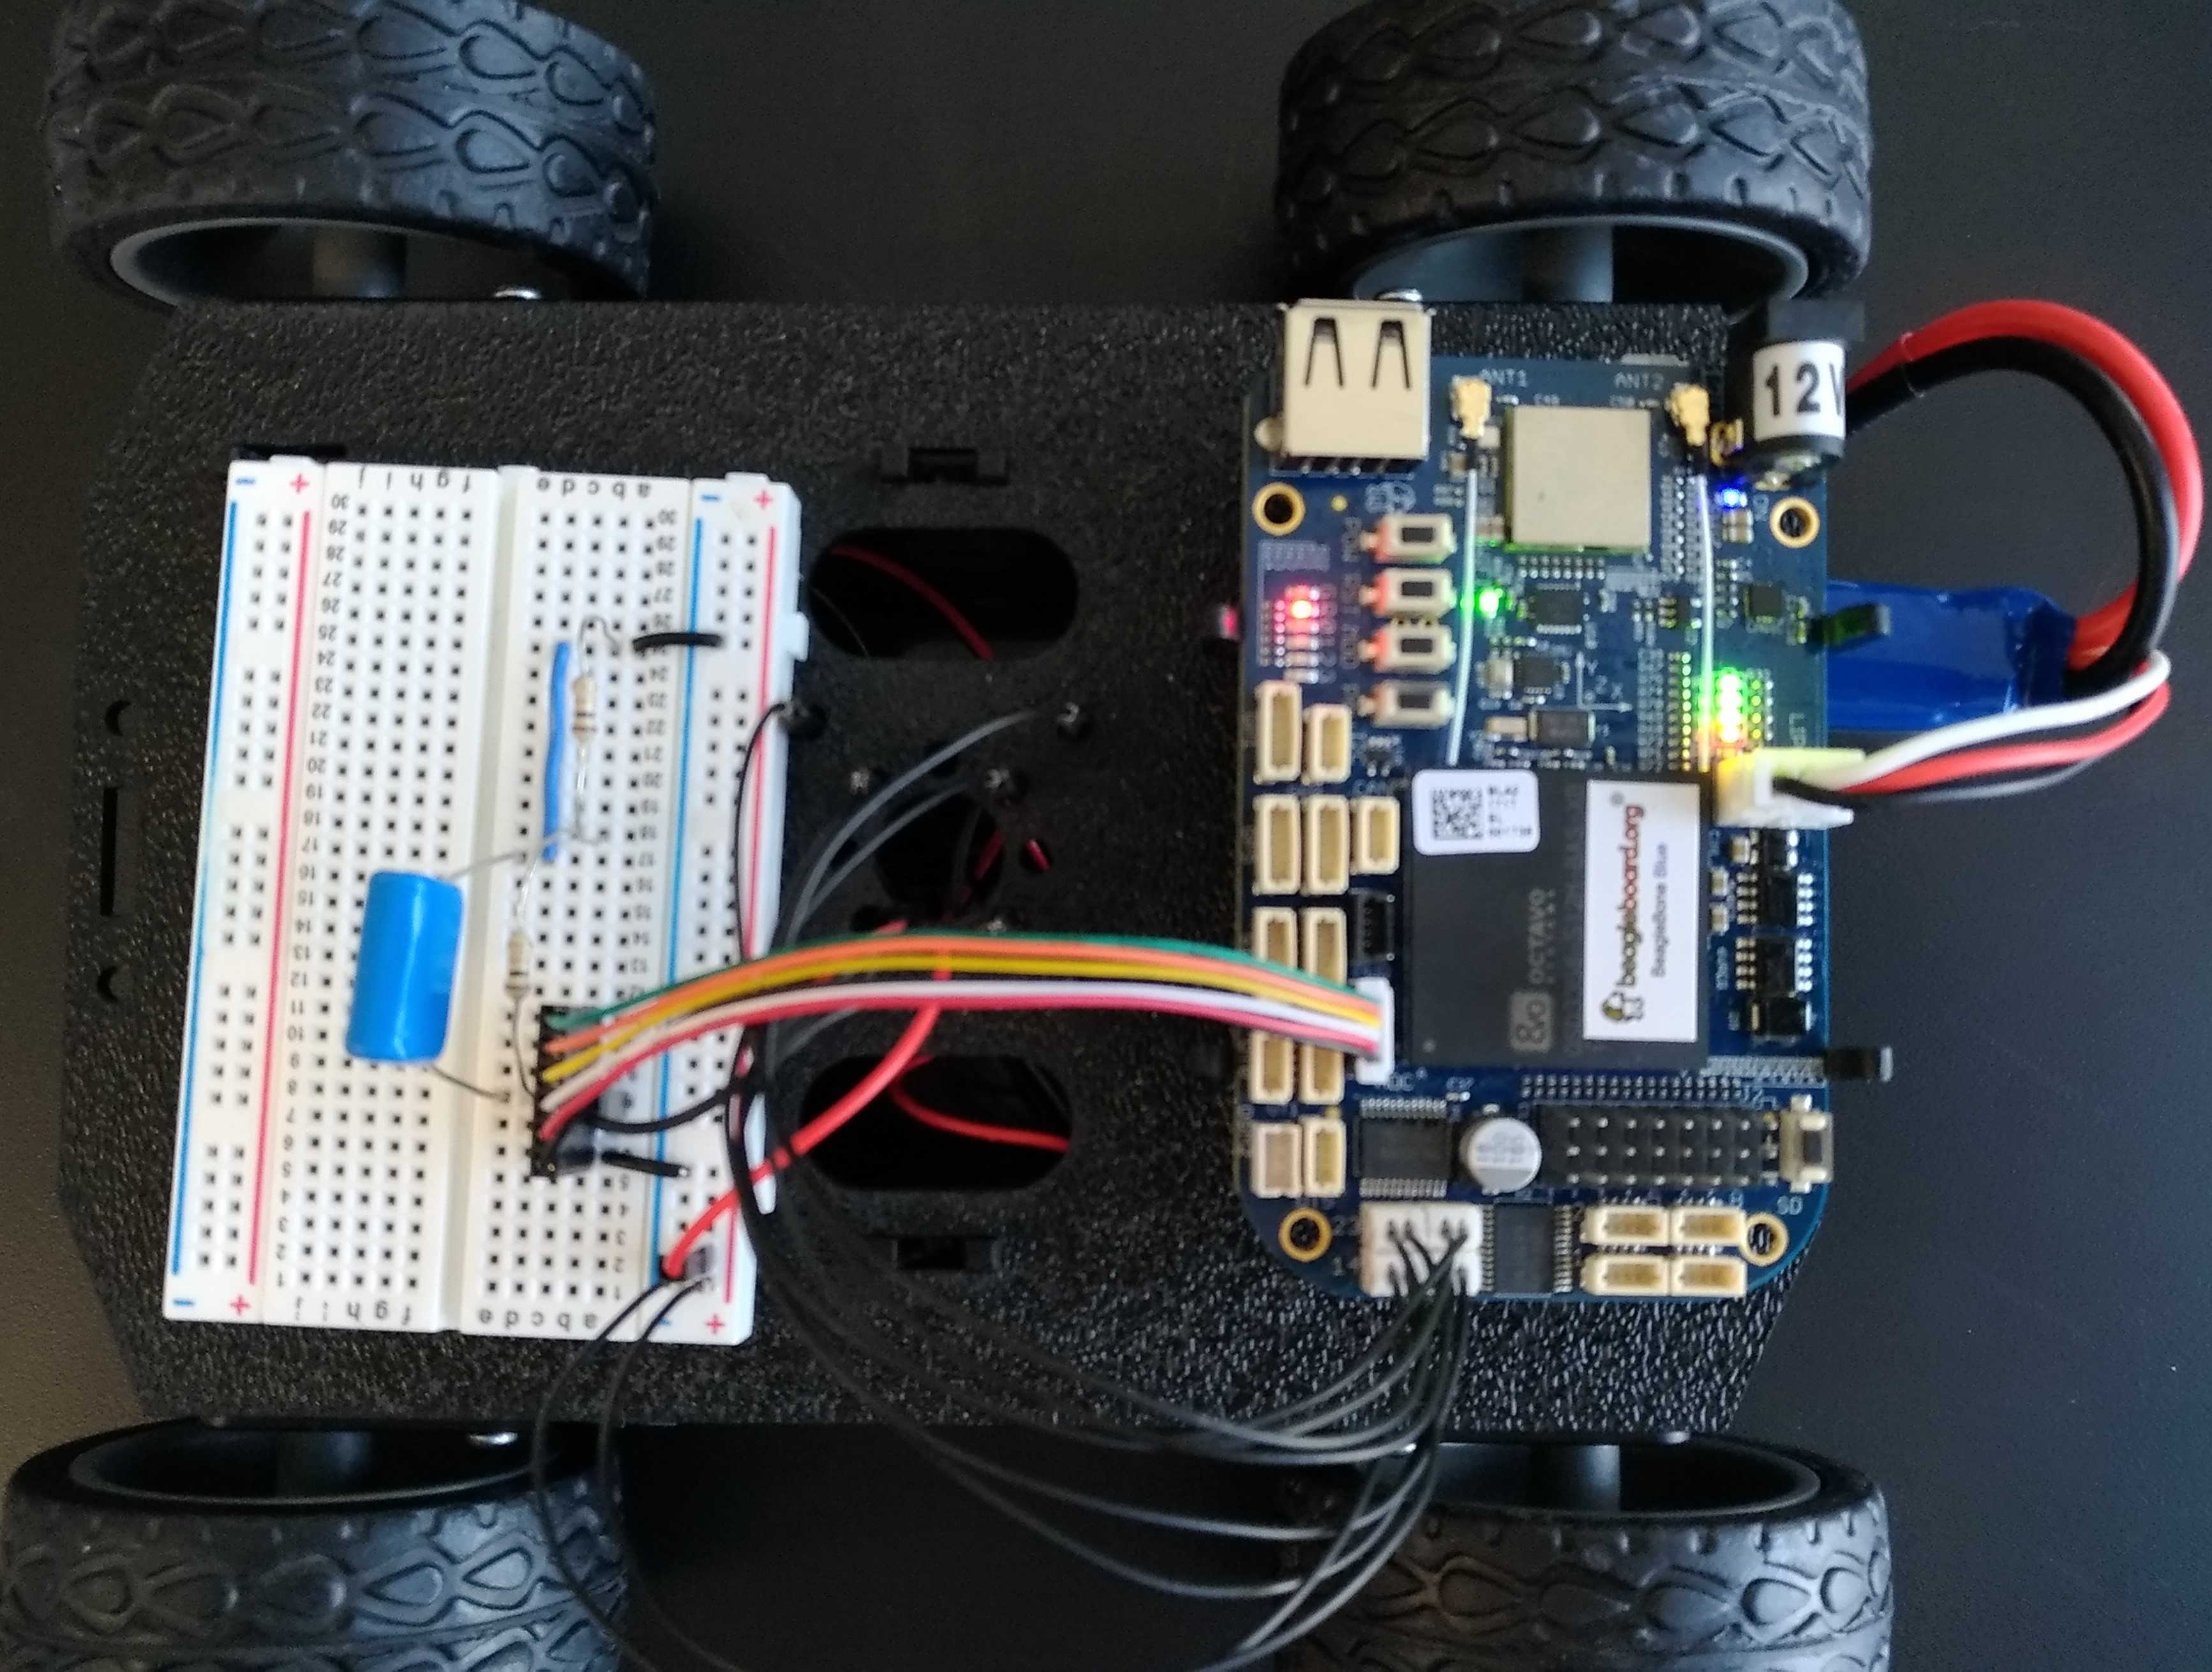
\includegraphics[scale=0.04]{figs/notConnectedSBC.jpg}
            \caption{Embedded Computer Not Connected}
            \label{fig:not_connected_bb}
        \end{figure}
        
        \begin{figure}
            \centering
            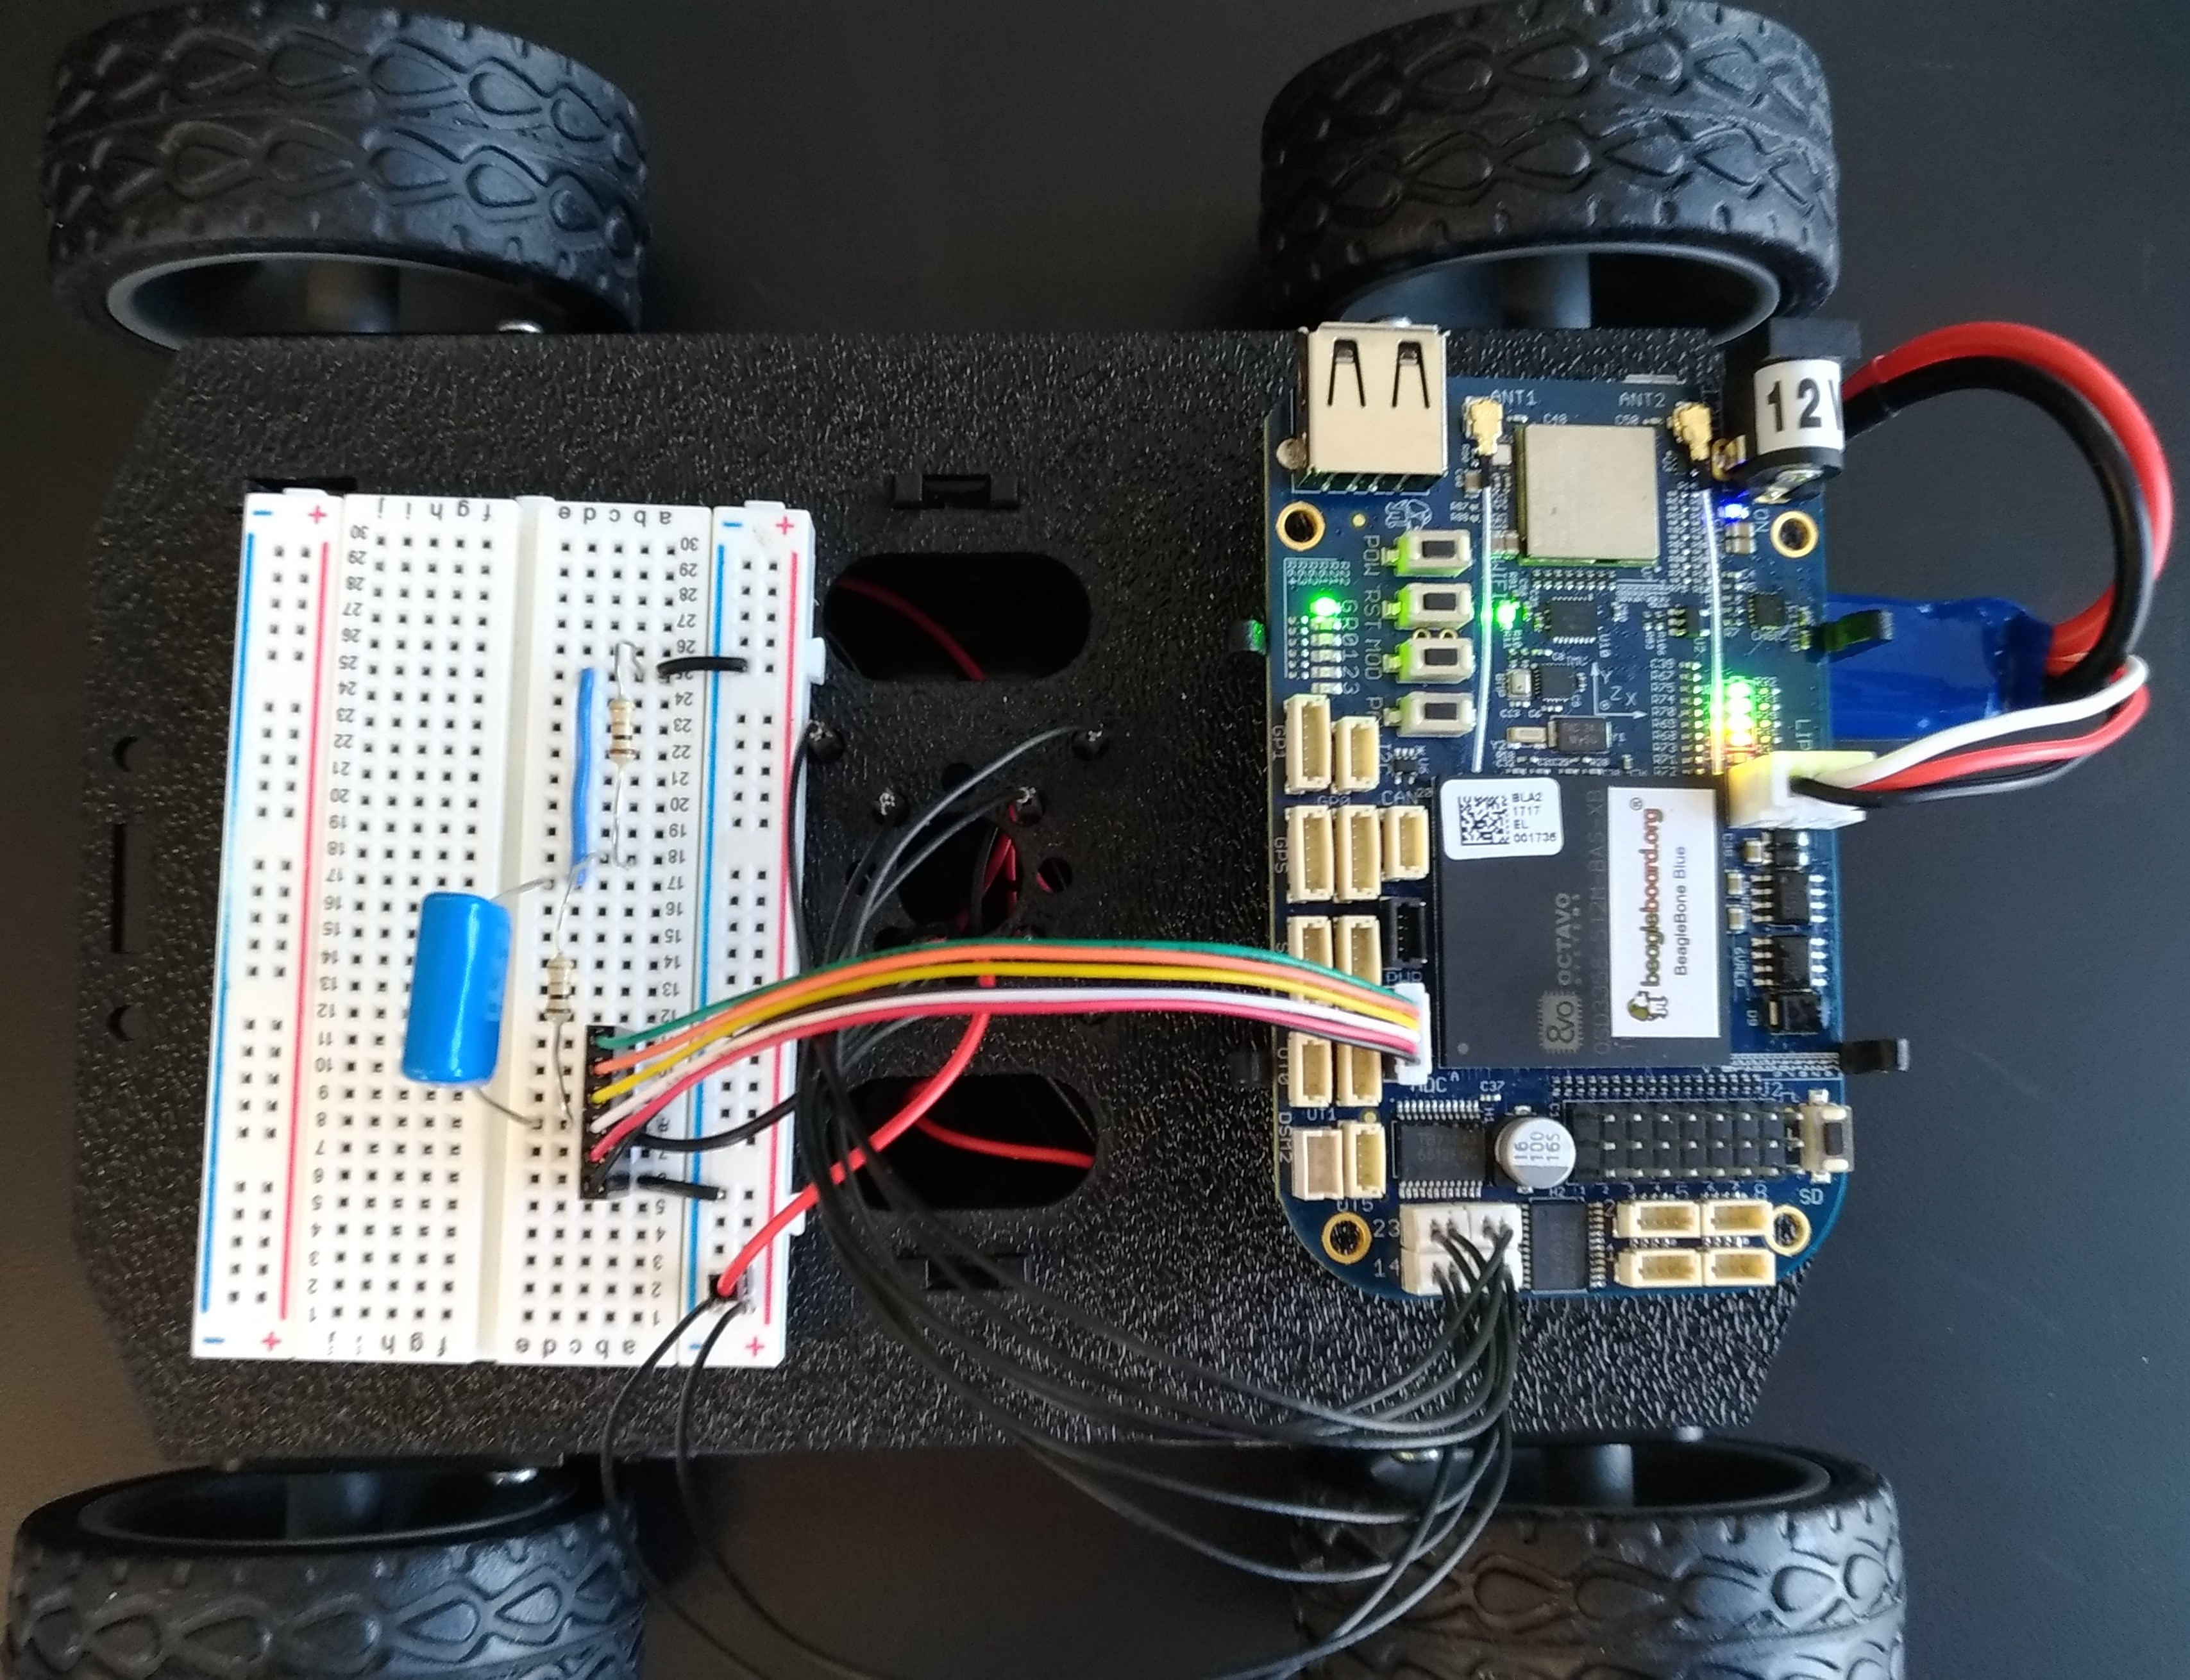
\includegraphics[scale=0.04]{figs/connectedSBC.jpg}
            \caption{Embedded Computer Connected}
            \label{fig:connected_bb}
        \end{figure}
    \end{multicols}
    \begin{block}{}
      \begin{small}
        \begin{itemize}
            \item Embedded computer accepts control commands and sends data to the server
            \item Red LED indicates the embedded computer is not connected and green LED indicates the embedded computer is connected
        \end{itemize}
      \end{small}
    \end{block}
\end{frame}

\begin{frame}{WeMo Insight Switch}{} % Elliot 
    \begin{columns}
    \column{0.5\textwidth}
      \begin{figure}
        \centering
        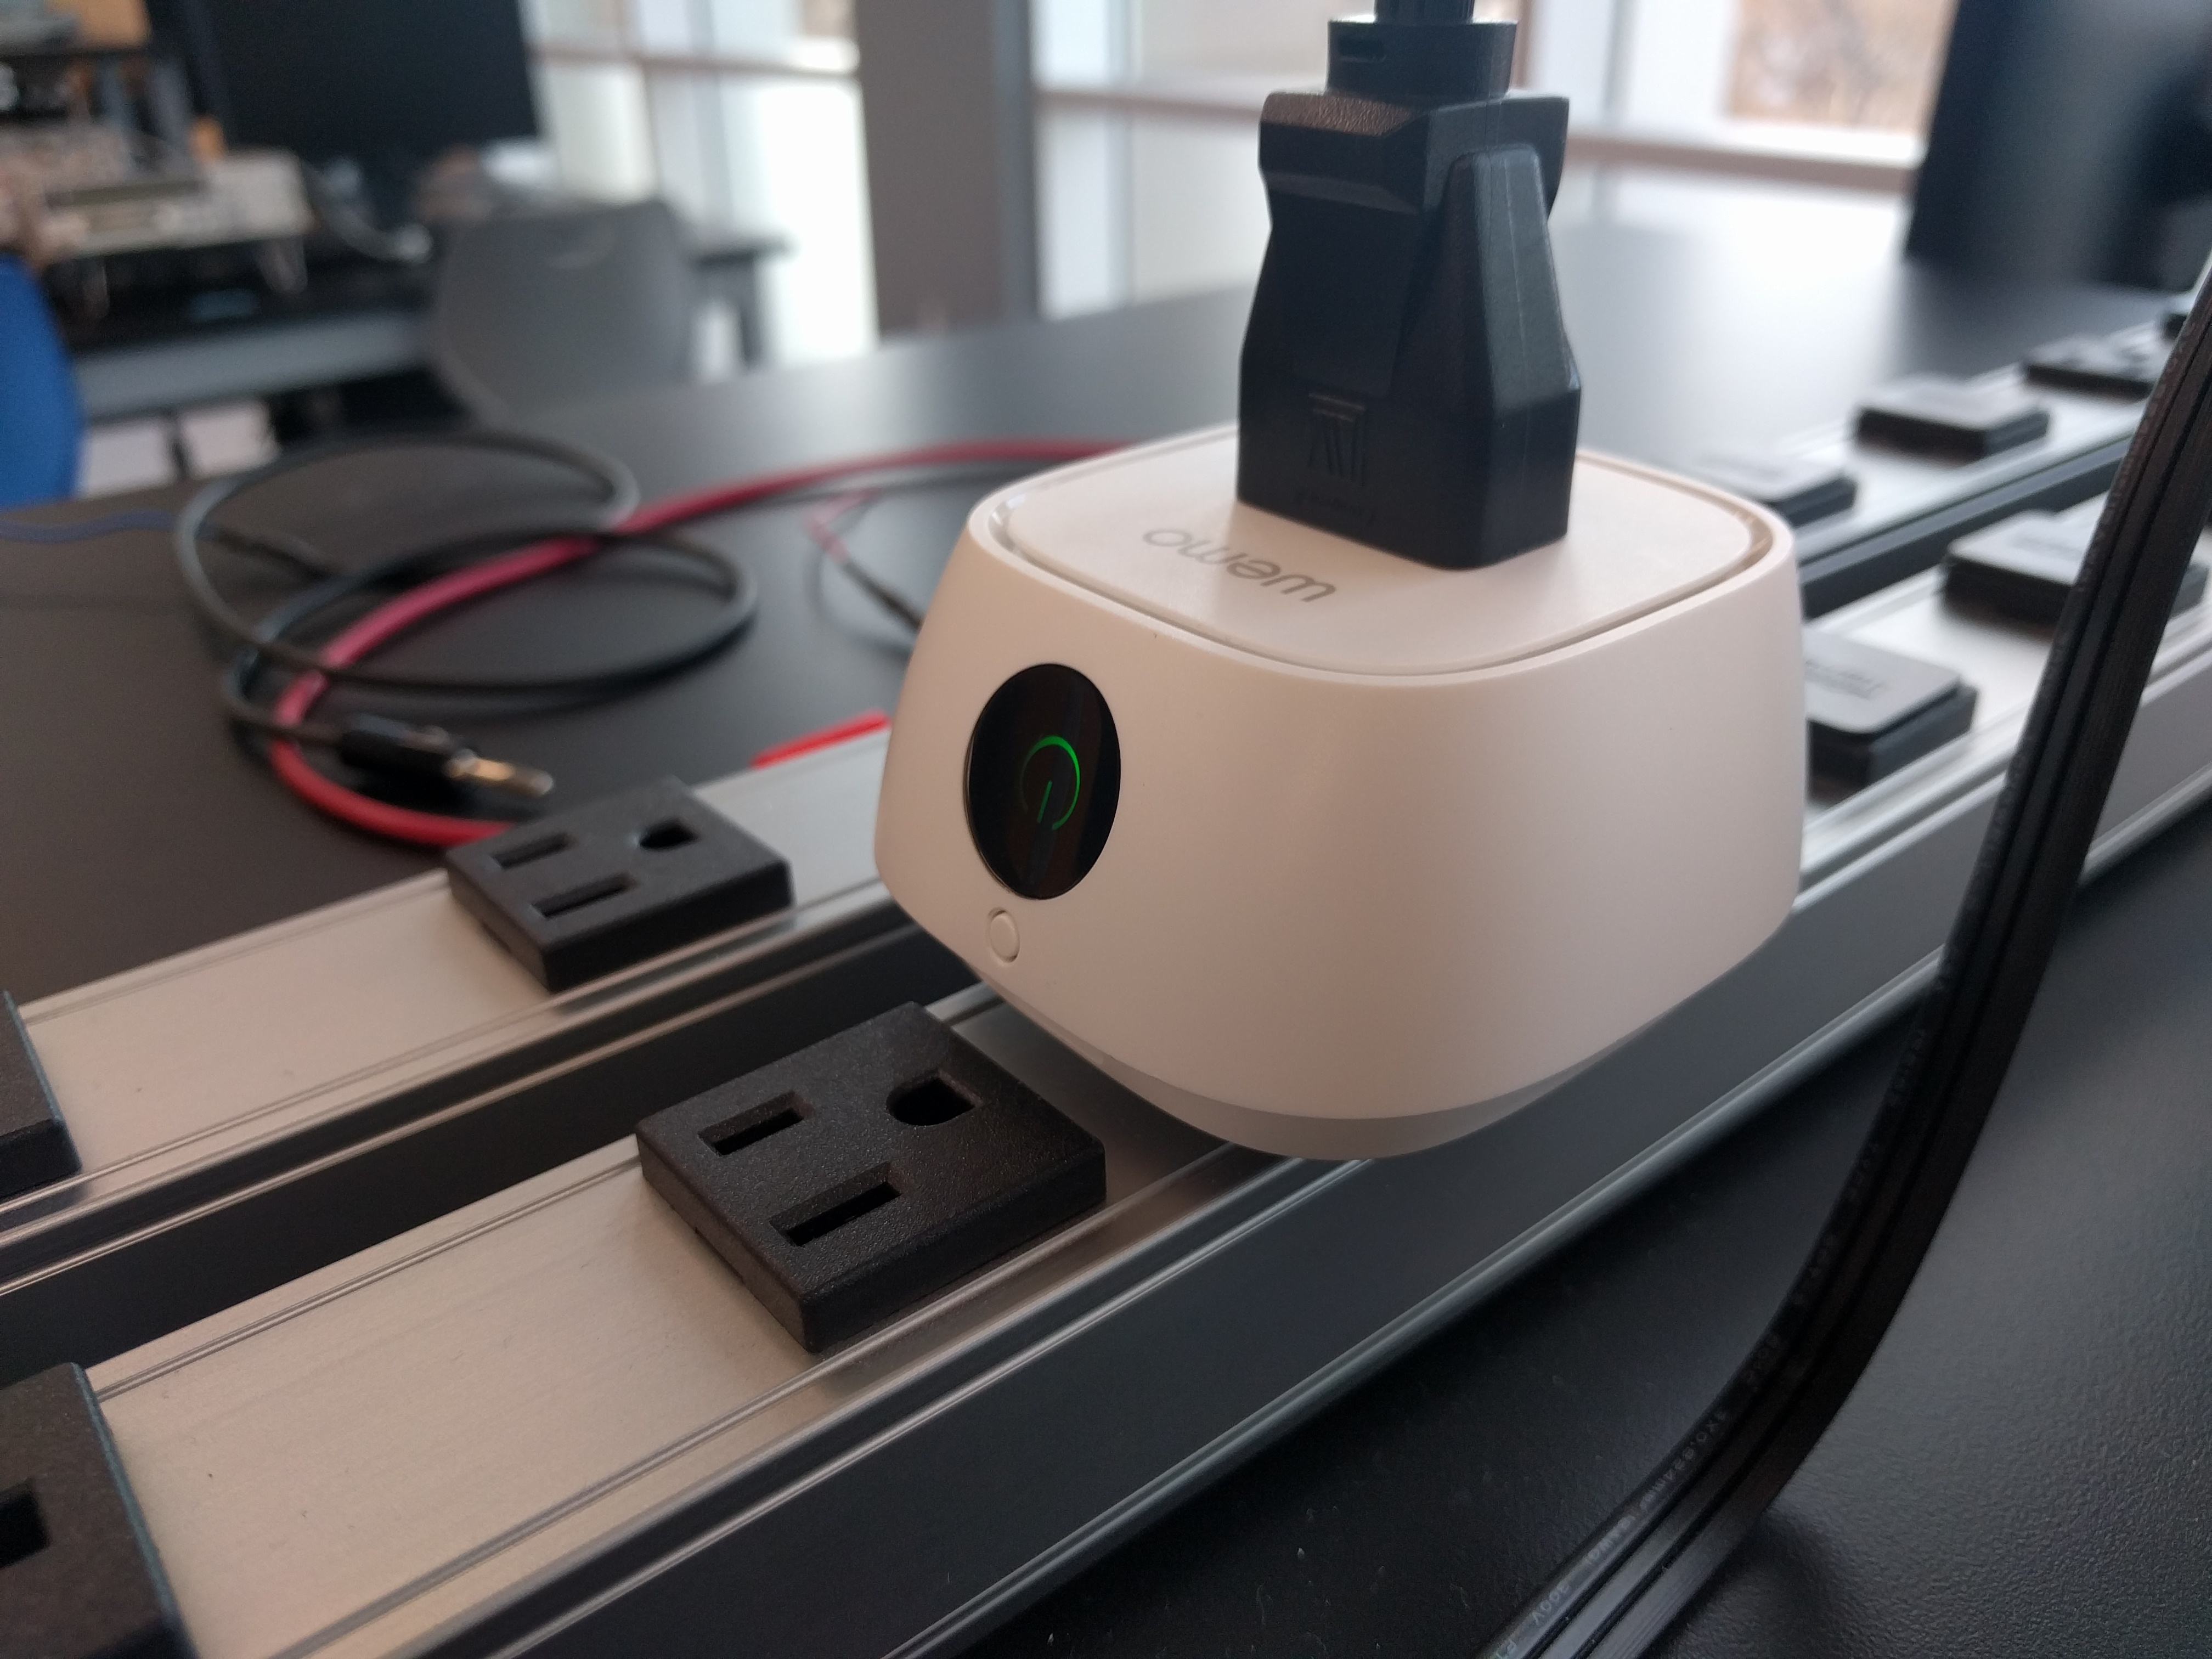
\includegraphics[scale=0.045]{figs/wemoView.jpg}
        \caption{WeMo Insight Smart Plug}
        \label{fig:wemo}
      \end{figure}
    \column{0.4\textwidth}
     \begin{block}{}
        \begin{itemize}
            \item Appliance is plugged into the WeMo Switch
            \item WeMo Switch can internally turn power on and off
            \item iBEMS will control the WeMo Switch remotely
        \end{itemize}
     \end{block}
    \end{columns}
\end{frame}

% \section{Overall Experimental Setup}
\begin{frame}{Overall Experimental Setup}{} % Elliot 
    \begin{figure}
        \centering
        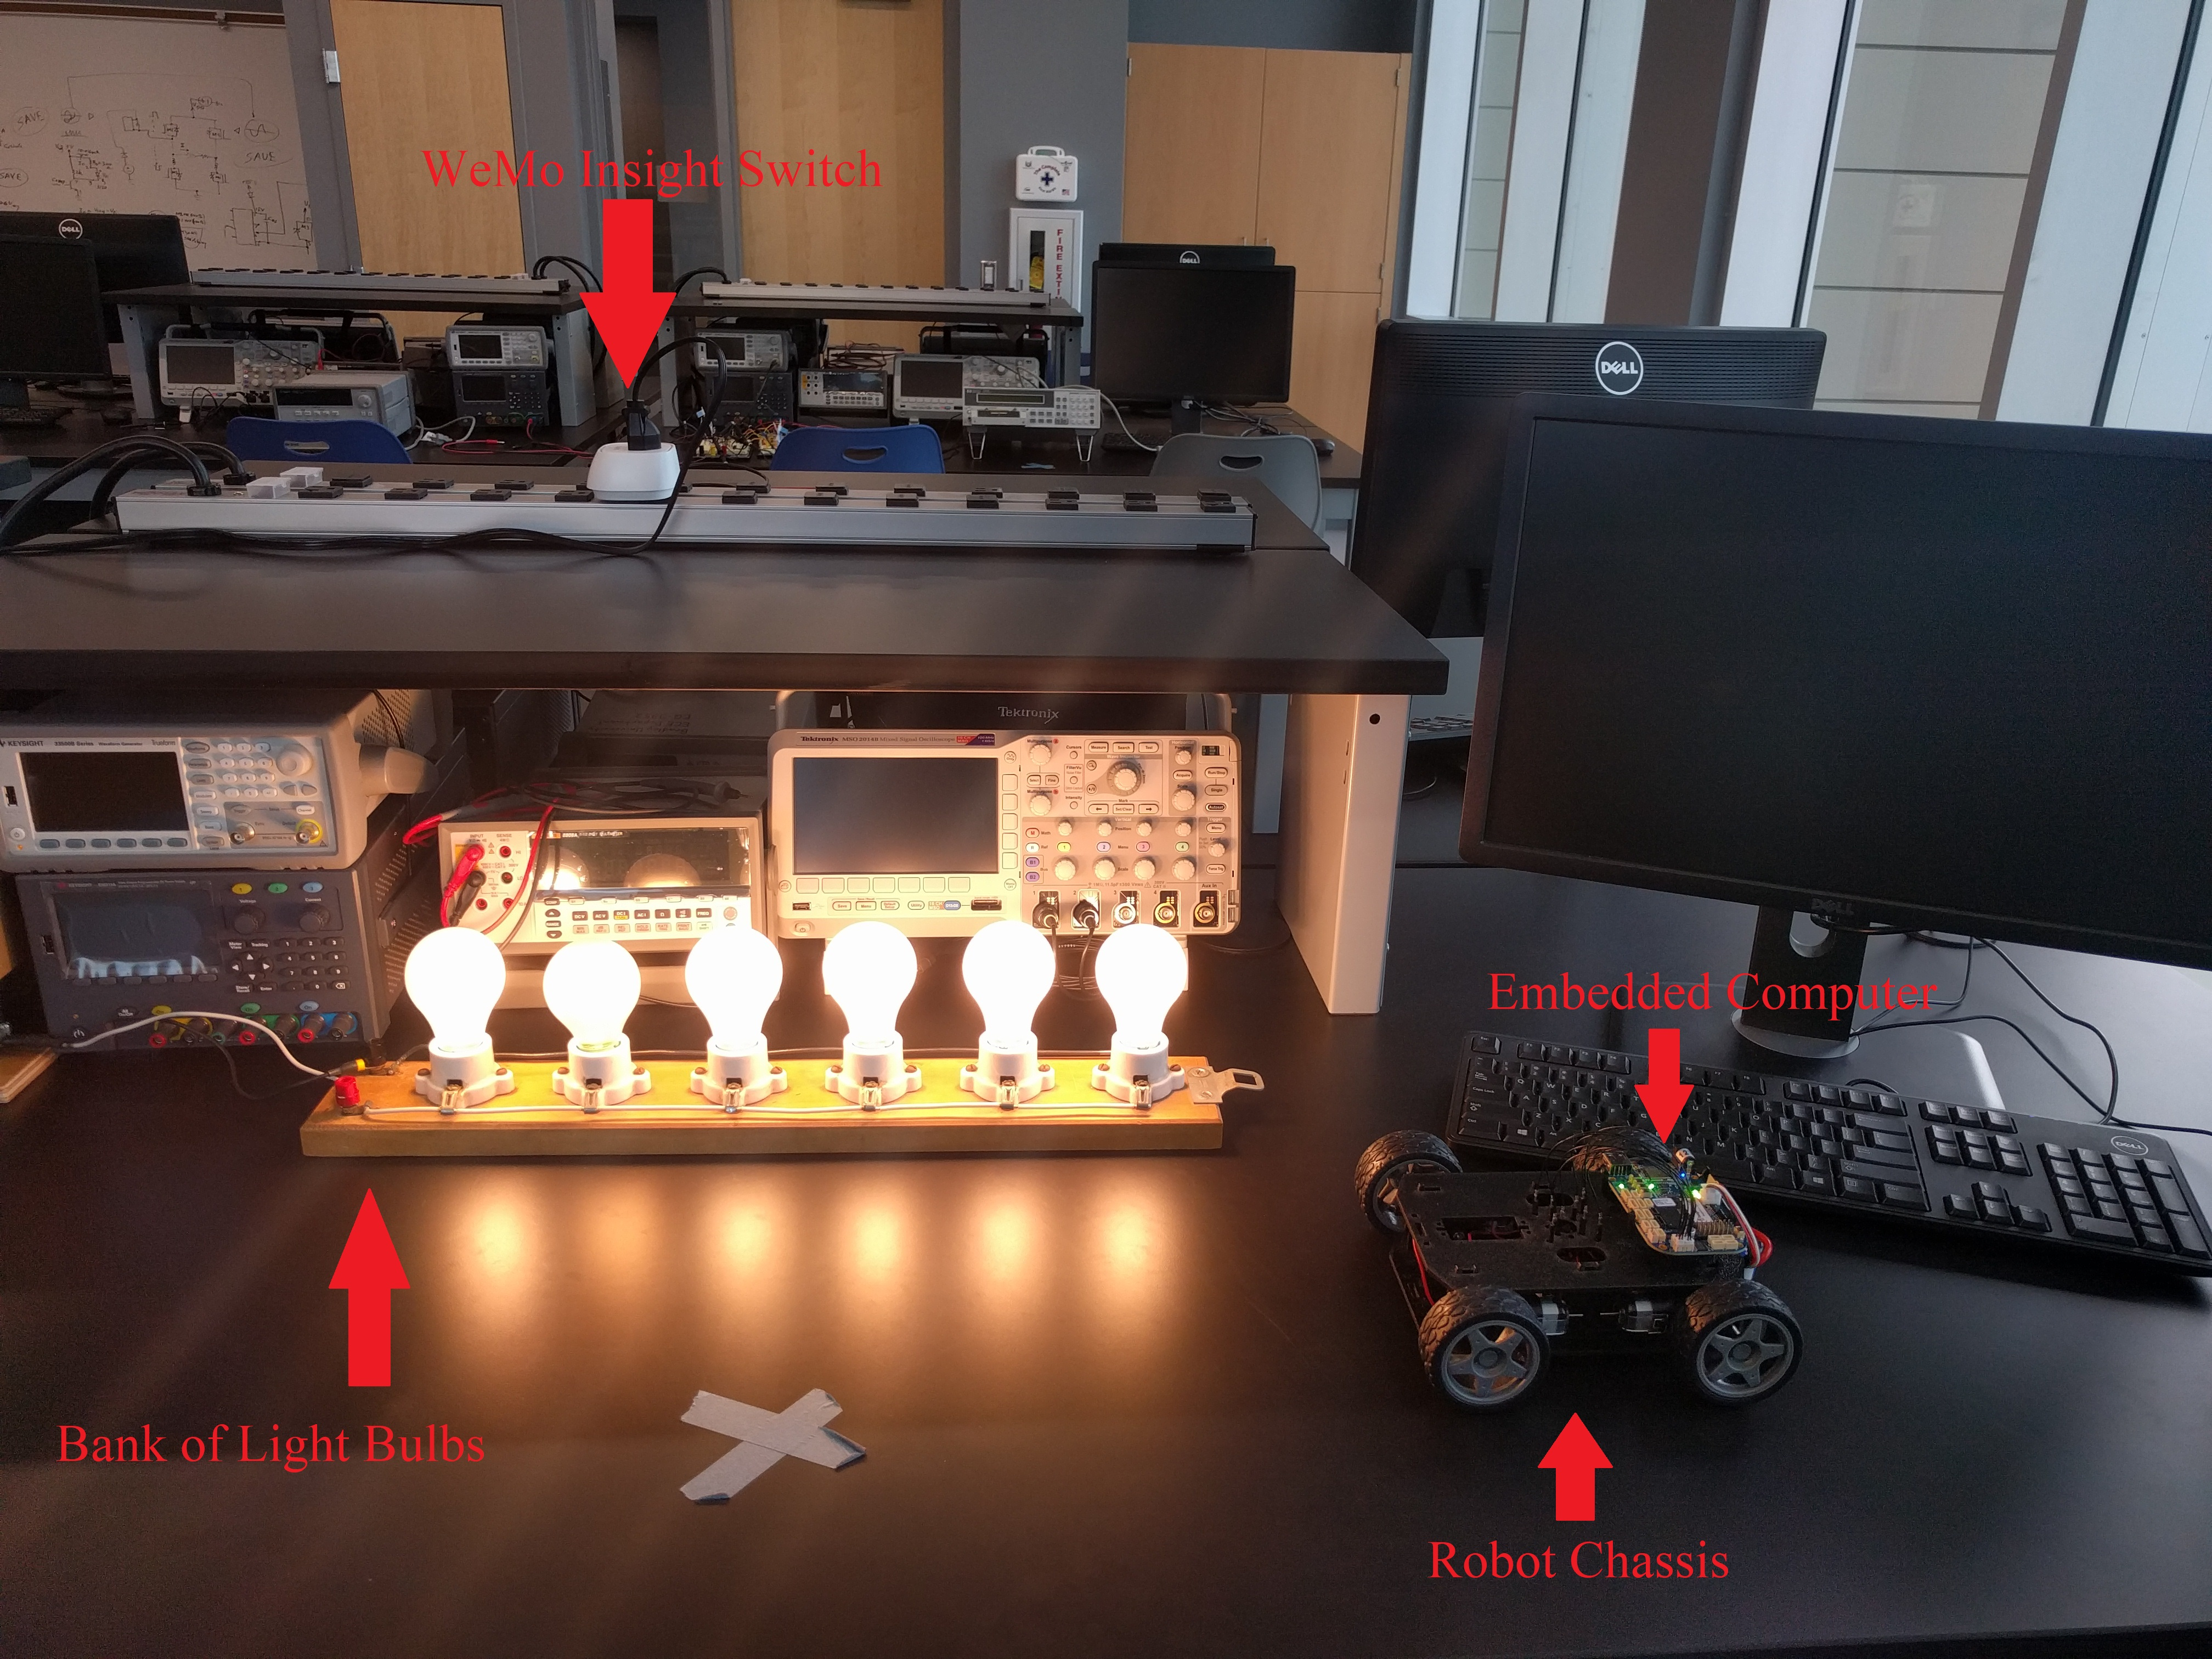
\includegraphics[scale=0.04]{figs/overallView.jpg}
        \caption{Overall View}
        \label{fig:my_label}
    \end{figure}
    \begin{block}{}
      Tested the WeMo Insight Switch with a bank of lights and the embedded computer with a robot chassis
    \end{block}
\end{frame}

\section{Software Implementation}

\begin{frame}{Control Agent Functionality}{}
    \begin{figure}
        \centering
        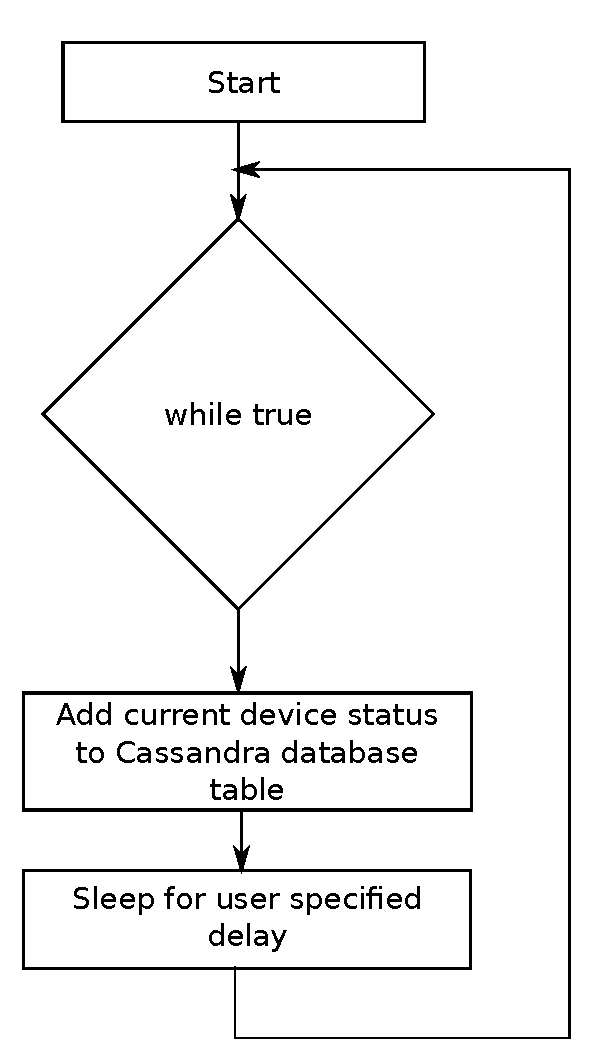
\includegraphics[scale=0.3]{figs/periodicQueryBehaviorFlow.pdf}
        \caption{periodicQueryBehavior Flow Chart}
        \label{fig:periodicQueryBehavior}
    \end{figure}
\end{frame}

\begin{frame}{Discovery Agent Functionality}{}
    \begin{figure}
        \centering
        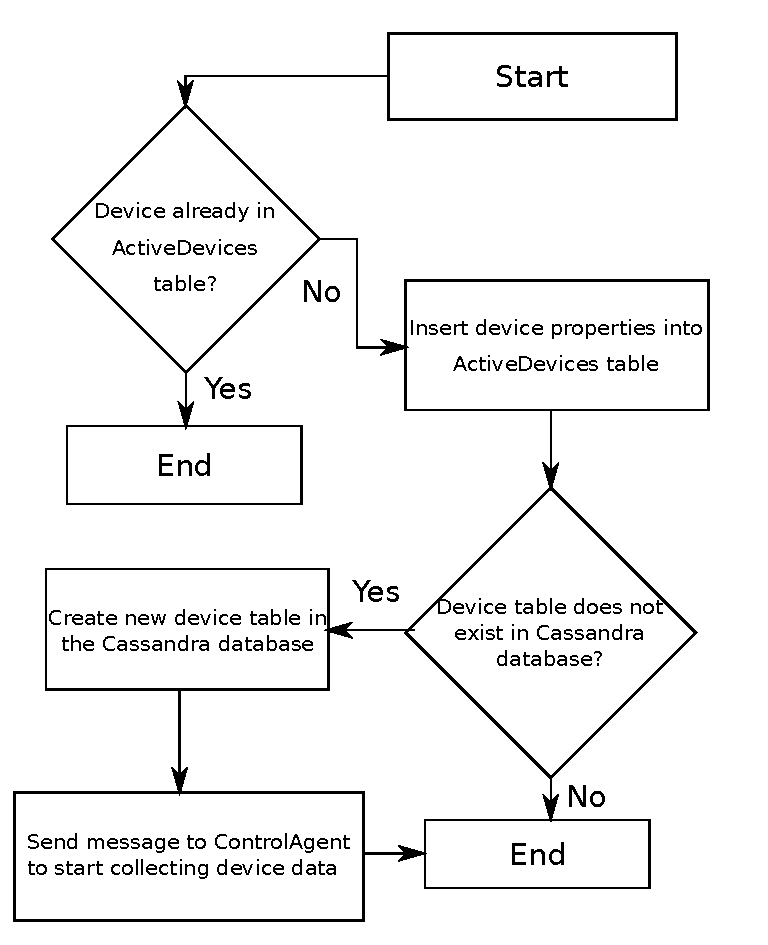
\includegraphics[scale=0.4]{figs/setDeviceToActiveFlow.pdf}
        \caption{setDeviceToActive Flow Chart}
        \label{fig:setDeviceToActive}
    \end{figure}
\end{frame}

\begin{frame}{Discovery Agent Functionality}{}
    \begin{figure}
        \centering
        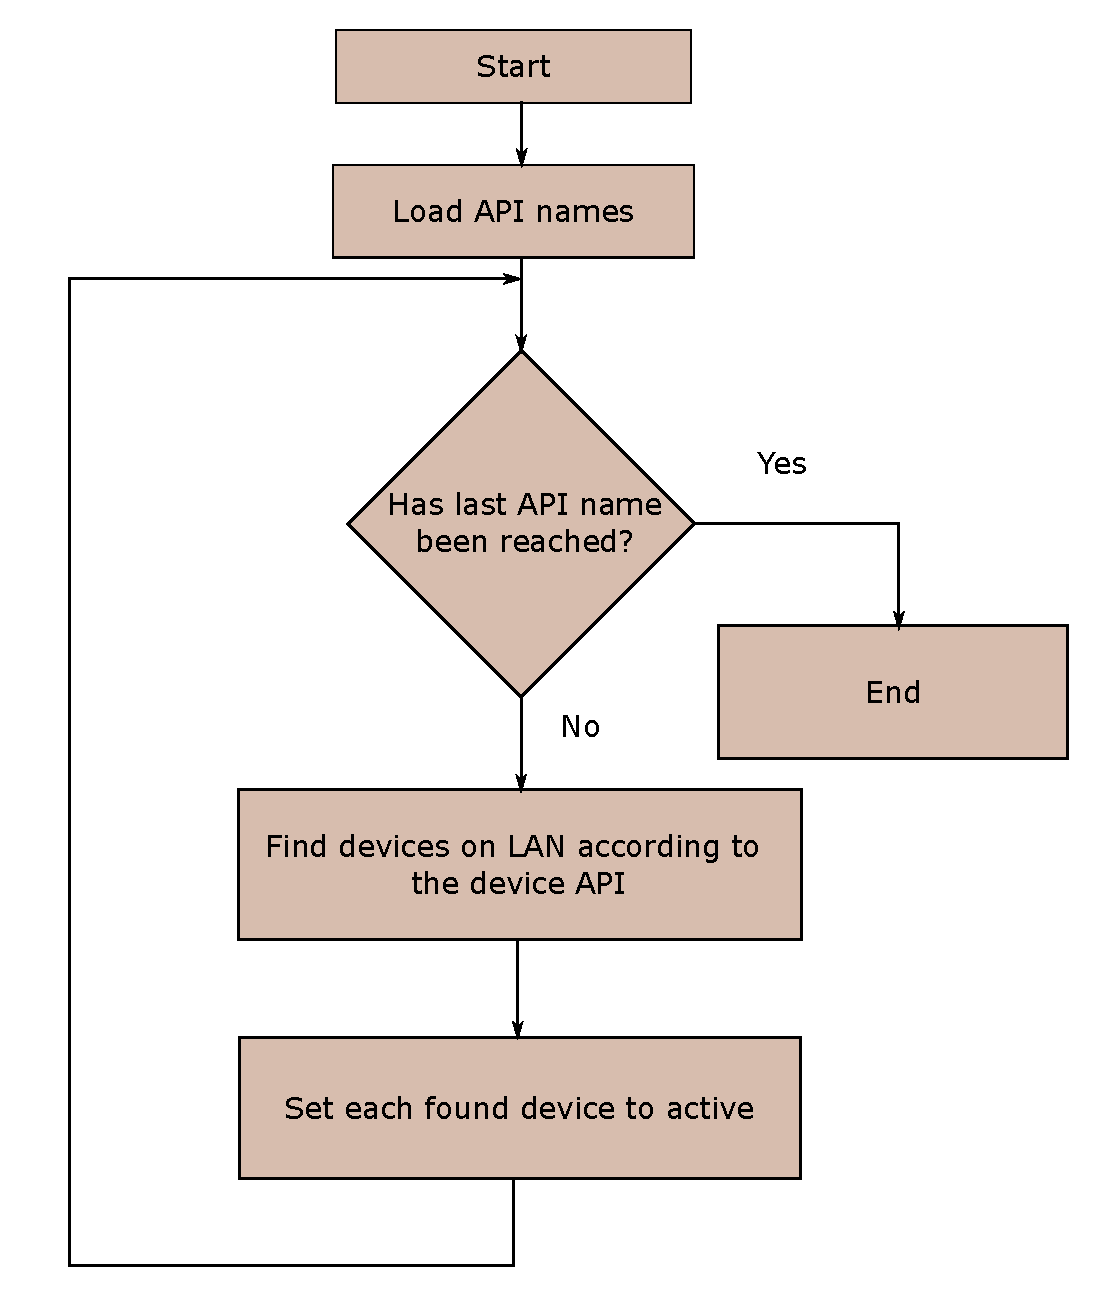
\includegraphics[scale=0.3]{figs/searchForDevicesFlow.pdf}
        \caption{searchForDevices Flow Chart}
        \label{fig:searchForDevices}
    \end{figure}
\end{frame}


\begin{frame}{Embedded Computer Receiver Program}{}
    \begin{figure}
        \centering
        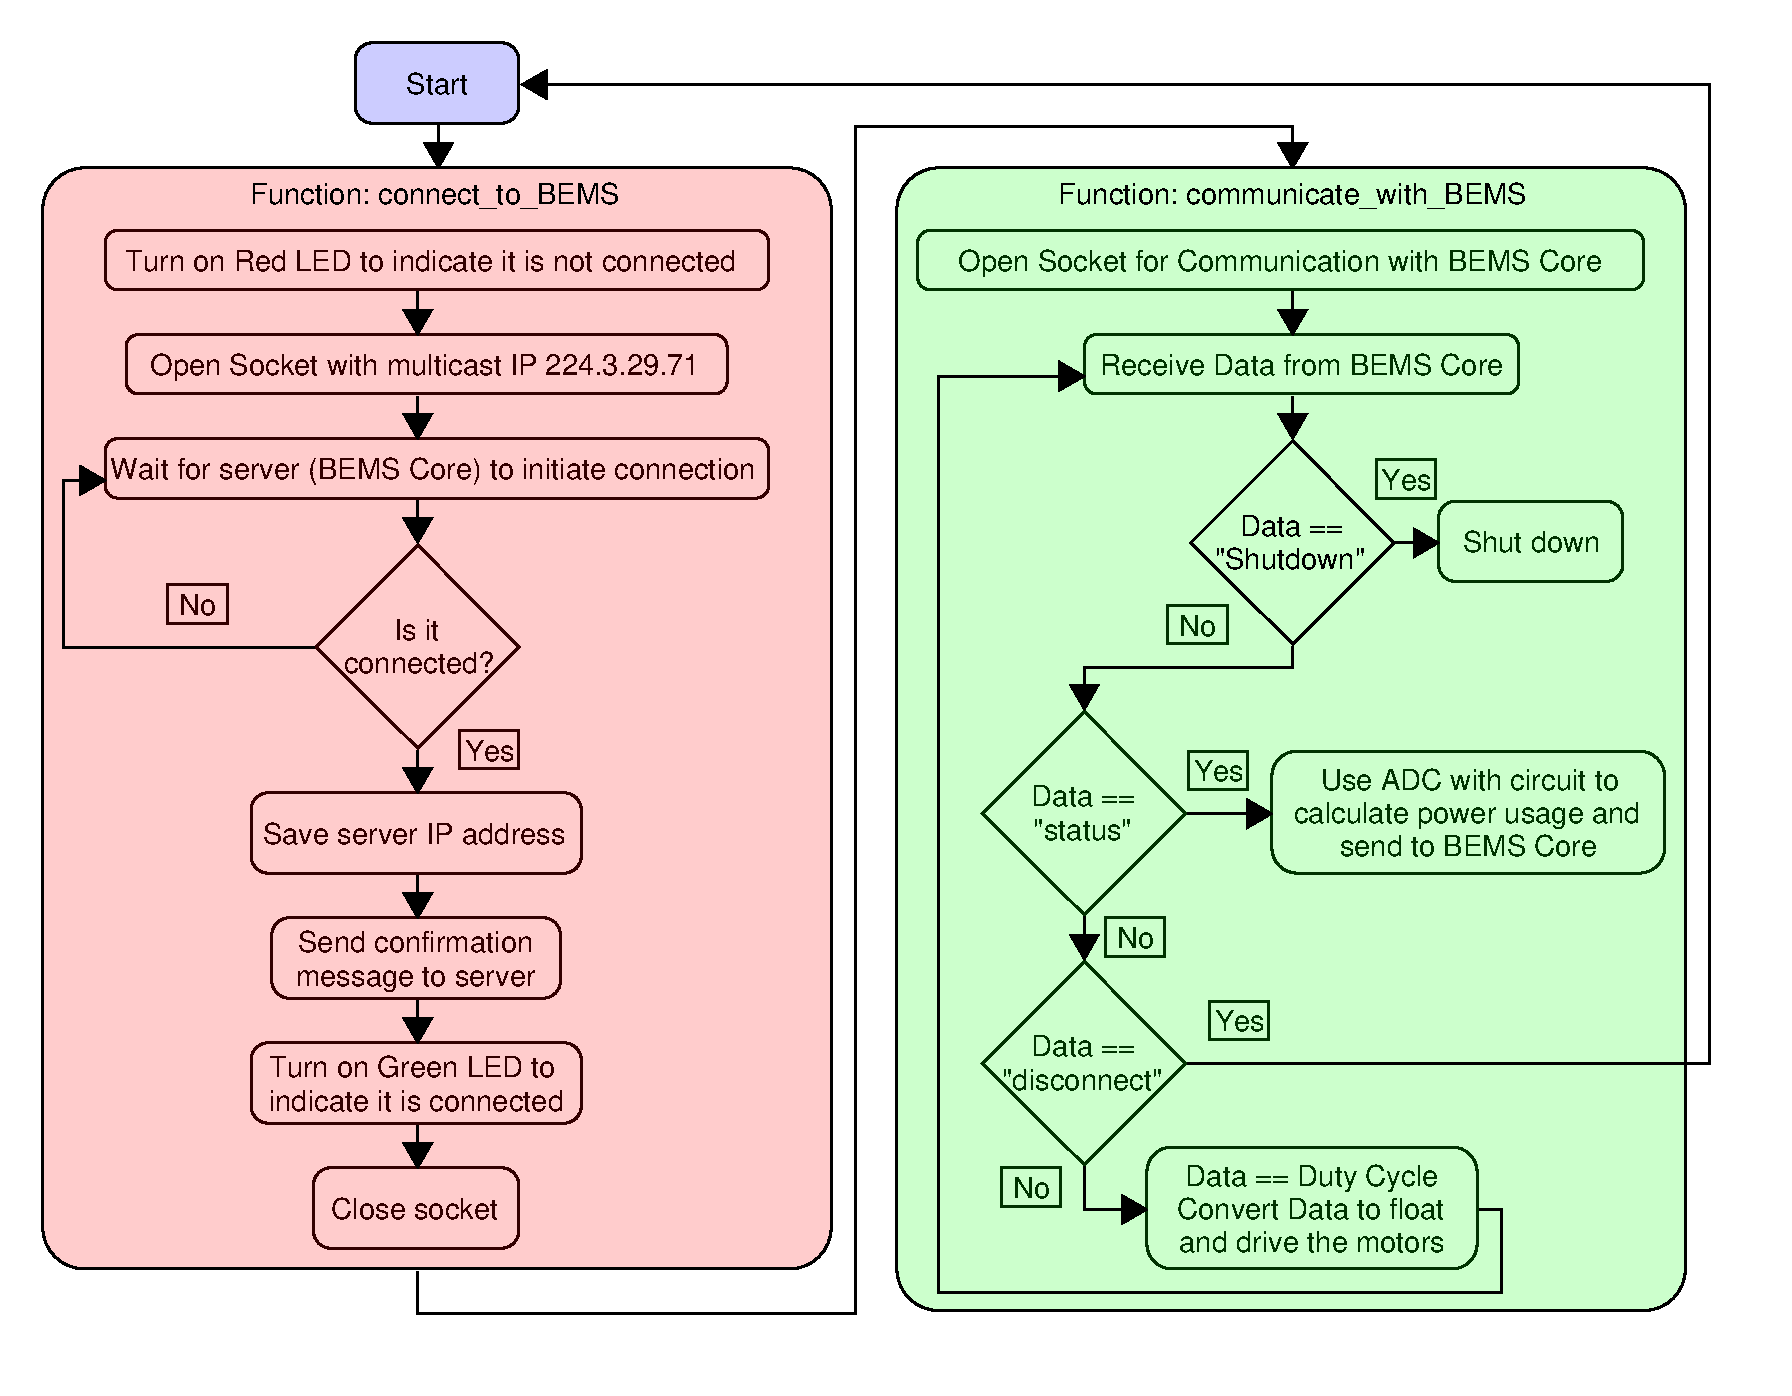
\includegraphics[scale=0.30]{figs/Beaglebone_Receiver_Diagram.pdf}
        \caption{Receiver Running on Embedded Computer}
        \label{fig:Beaglebone_Receiver_Diagram}
    \end{figure}
\end{frame}

\begin{frame}{Startup Menu}
    \begin{multicols}{2}
        \begin{figure}
            \centering
            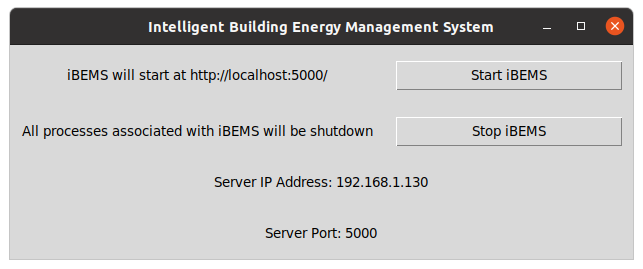
\includegraphics[scale=0.2]{figs/BEMS_GUI_Linux.png}
            \caption{Desktop GUI}
            \label{fig:desktopgui}
        \end{figure}
        \begin{figure}
            \centering
            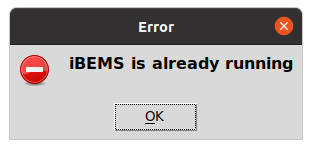
\includegraphics[scale=0.35]{figs/BEMS_GUI_Linux_Warning.png}
            \caption{Popup Error}
            \label{fig:popuperror}
        \end{figure}
    \end{multicols}
    \begin{block}{}
      \begin{itemize}
        \item Clicking "Start iBEMS" will lauch the web server and all 3 agents as well as launch the computer's web browser and load the login page automatically
        \item If the user accidentally clicks "Start iBEMS" while it already running, a warning message will appear to prevent errors
        \item Clicking "Stop iBEMS" will stop the web server and agents and close the web browser
    \end{itemize}
    \end{block}
\end{frame}

\begin{frame}{Startup Menu Functions}{}
    \begin{figure}
        \centering
        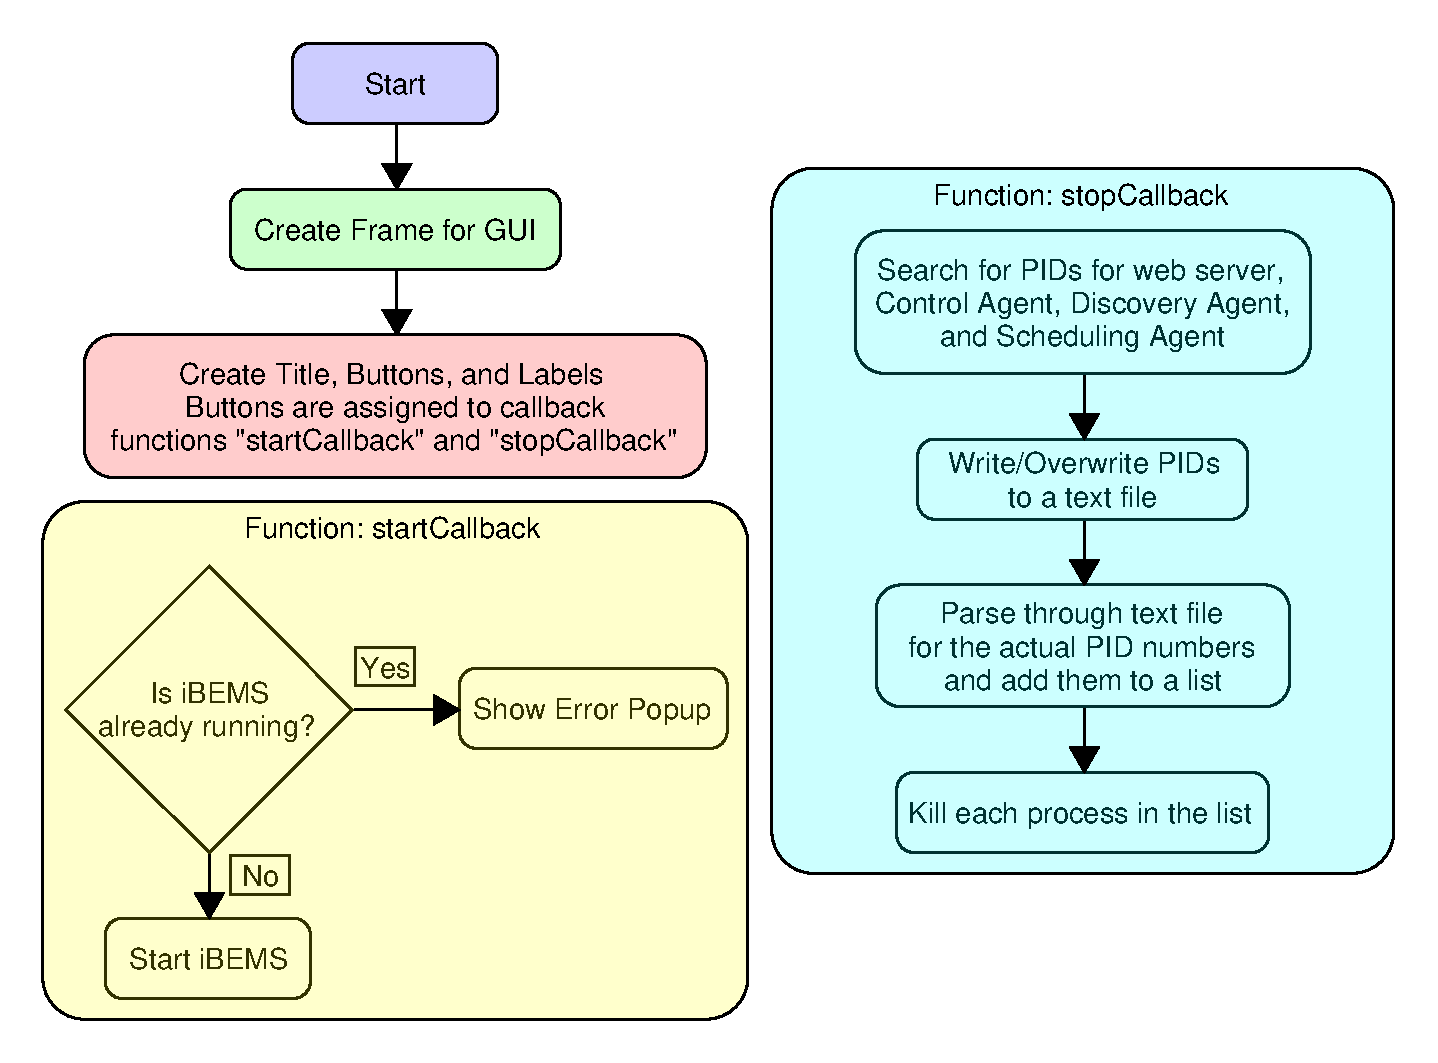
\includegraphics[scale=0.4]{figs/GUI_Diagram.pdf}
        \caption{Diagram for Startup Menu Functionality}
        \label{fig:GUI_Diagram}
    \end{figure}
\end{frame}

% System Architecture Diagram
\begin{frame}{Home Page}{} % Brian
    % High-Level Architecture Figure
    \begin{figure}
        \centering
        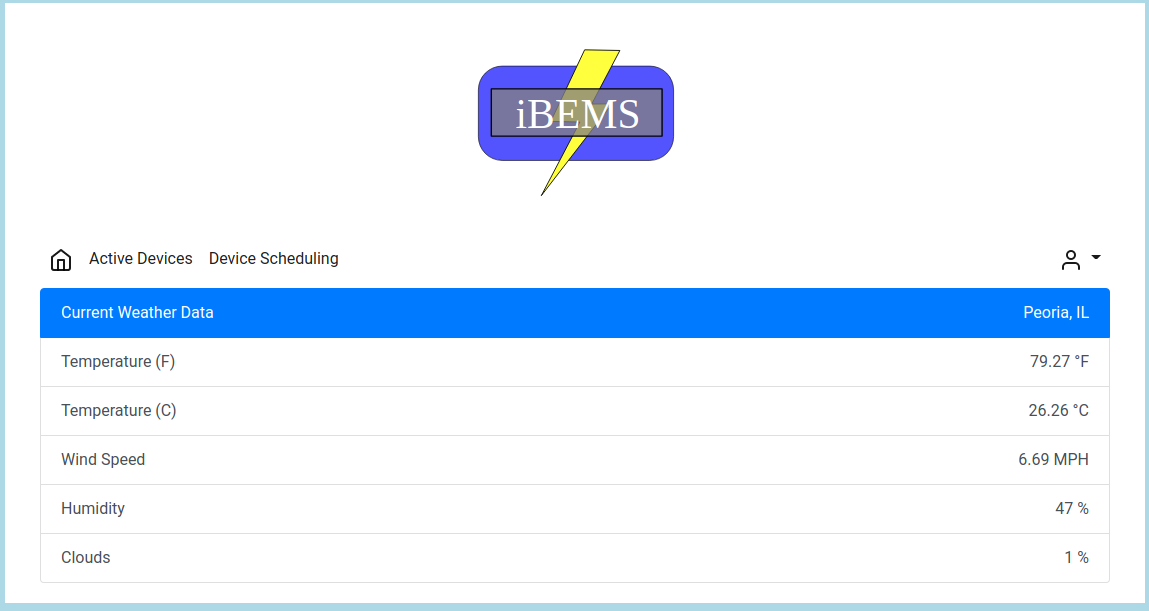
\includegraphics[scale=0.2]{figs/Home_screen.png}
        \caption{Home Screen}
        \label{fig:Home_screen}
    \end{figure}
    \begin{block}{}
      \begin{small}
        \begin{itemize}
        \item This will be loaded when iBEMS is first booted and it simply shows some current data about the weather 
        \item The Home Page is also accessible by clicking the Home Icon in the upper left corner
        \end{itemize}
      \end{small}
    \end{block}
\end{frame}

\begin{frame}{Active Devices Page}{} % Elliot 
    \begin{columns}
    \column{0.5\textwidth}
      \begin{figure}
            \centering
            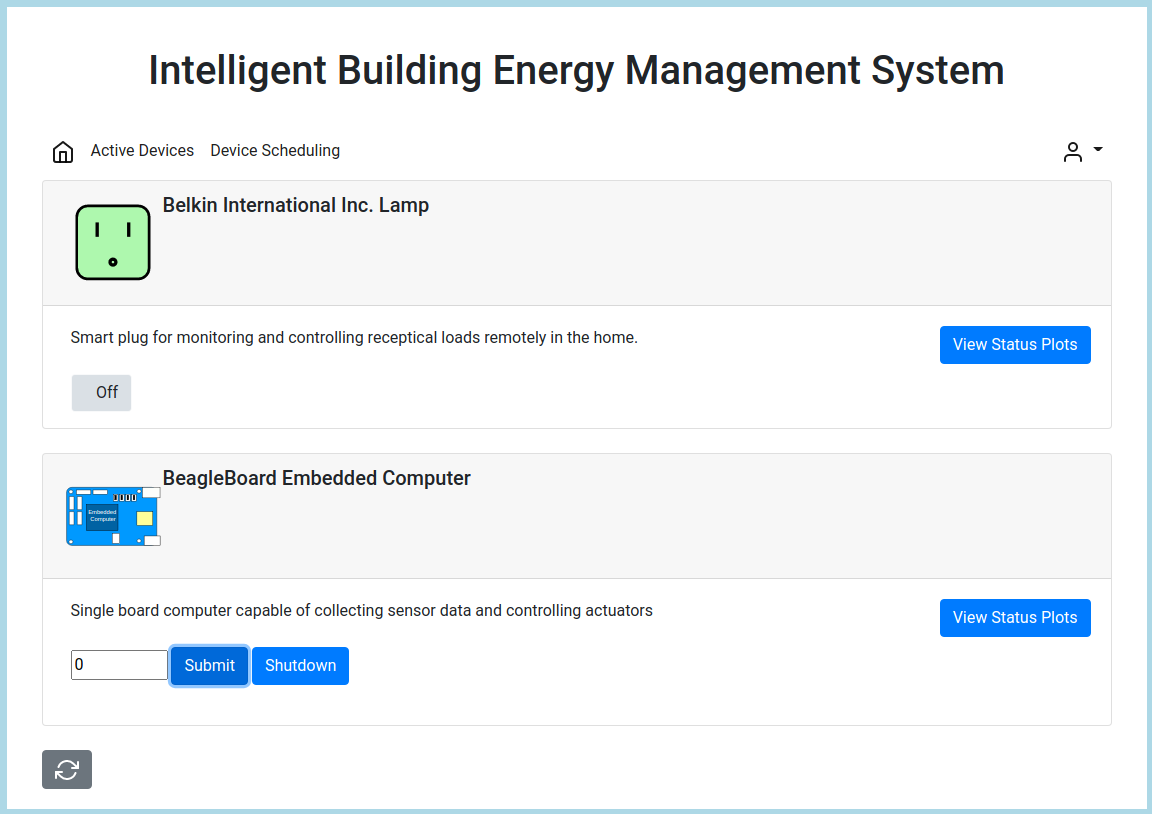
\includegraphics[scale=0.13]{figs/ActiveDevices_screen.png}
            \caption{Active Devices Page}
            \label{fig:active_devices}
        \end{figure}
    \column{0.45\textwidth}
        \begin{block}{}
          \begin{itemize}
            \item Page allows users to directly control available devices in real time
            \item WeMo Insight Smart Plug can be turned on and off
            \item PWM duty cycle of the embedded computer can be adjusted in increments of 0.1
        \end{itemize}
        \end{block}
    \end{columns}
\end{frame}

\begin{frame}{WeMo Power Plot}{} % Brian
    \begin{figure}
        \centering
        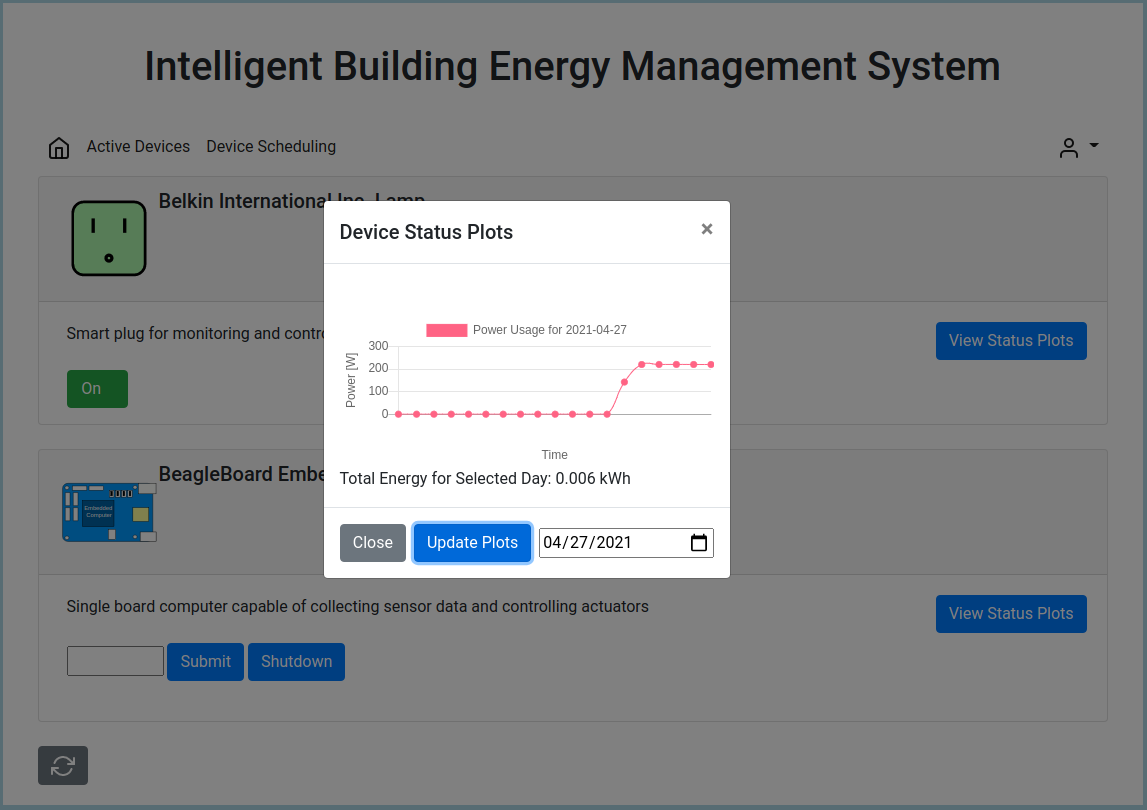
\includegraphics[scale=0.15]{figs/ActiveDevices_plot.png}
        \caption{Active Devices Plot}
        \label{fig:active_devices_plot}
    \end{figure}
    \begin{block}{}
      \begin{small}
        \begin{itemize}
            \item Clicking "View Status Plots" launches modal
            \item User can select any day and view the power usage
        \end{itemize}
      \end{small}
    \end{block}
\end{frame}

\begin{frame}{Scheduling/Applications Page}{} % Elliot 

    \begin{columns}
    \column{0.5\textwidth}
      \begin{figure}
            \centering
            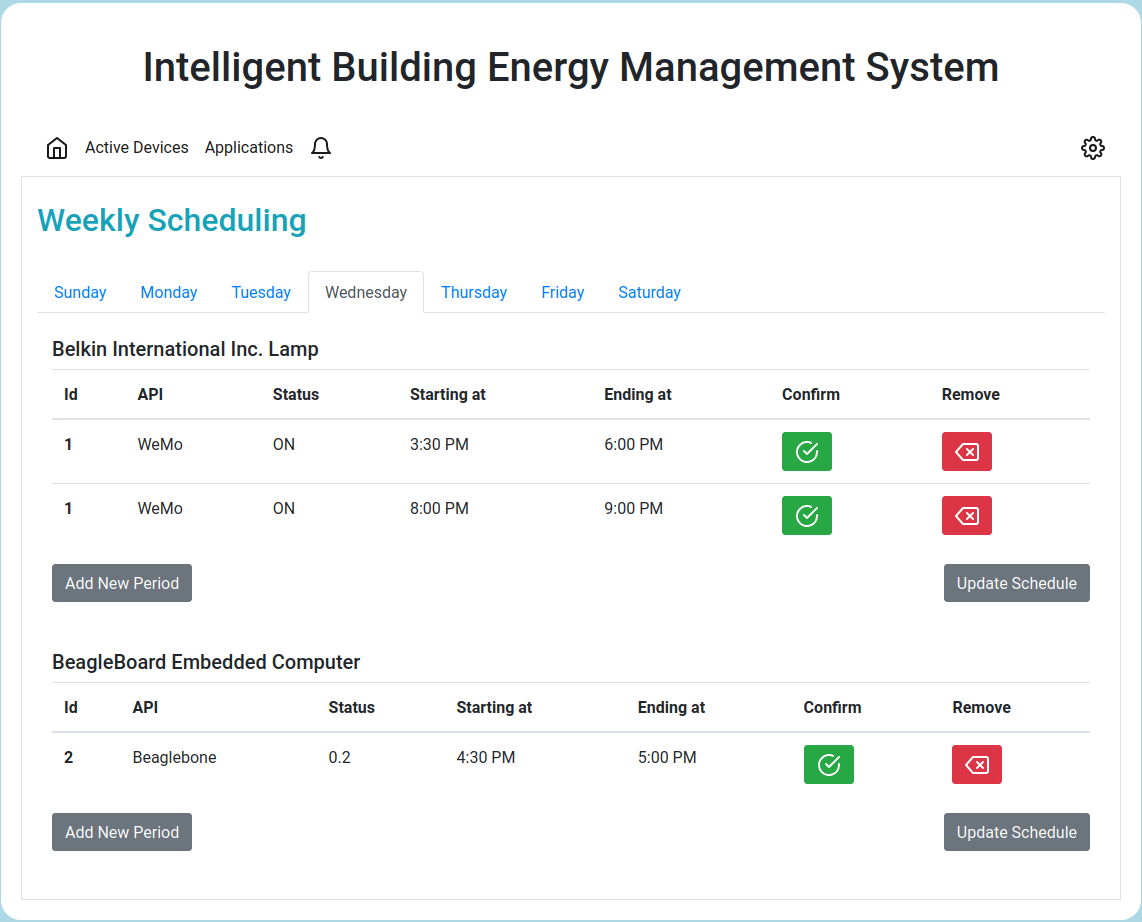
\includegraphics[scale=0.15]{figs/Applications_screen.png}
            \caption{Scheduling Page}
            \label{fig:schedulingl}
        \end{figure}
        \column{0.45\textwidth}
        \begin{block}{}
          \begin{itemize}
            \item Clicking on "Applications" on the nav bar loads the weekly scheduling feature
            \item User can input whatever times they want with devices to be in a specified state (on/off for WeMo plug and duty cycle for the embedded computer)
        \end{itemize}
        \end{block}
    \end{columns}
\end{frame}

\section{Conclusion}
\begin{frame}{Conclusion}{} % Elliot
  \begin{columns}
    \column{0.5\textwidth}
    \begin{figure}
      \centering
      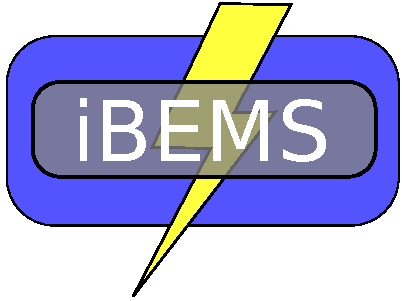
\includegraphics[scale=0.8]{figs/logo.pdf}
      \label{fig:logo}
    \end{figure}
    \column{0.45\textwidth}
    \begin{block}{}
      \begin{itemize}
      \item Advantages: open source, simple interface, modular agent-based code base
      \item Disadvantages: can only operate on a LAN, lacks features of a commercial BEMS system
      \item Challenges: adapting the platform for an enterprise network in a commercial building, security features 
    \end{itemize}
    \end{block}
  \end{columns}  
\end{frame}

\begin{frame}{Conclusion}{}
  \begin{block}{Further Improvements}
    \begin{itemize}
    \item Refactor the user interface
    \item Granular user access control
    \item Refactor agent communication
    \item Intelligent algorithms
    \item Mobile app
    \item Persistent device information storage
    \end{itemize}
  \end{block}
\end{frame}




\end{document}



%%% Local Variables:
%%% mode: latex
%%% TeX-master: t
%%% End:
